\section{第五章\ 飞升入定：将游戏世界部署到云端}
% 张道平

在第四章中，我们把游戏后端从单机推进到了分布式架构：数据库分片突破了存储瓶颈，负载均衡分发玩家请求，协调服务器实现跨服通信，健康检查监控节点状态。从逻辑上看，一个能承载数千人同时在线的多服协同系统已经成型。

然而，架构图画得再漂亮，最终都要落到真实的机器上运行。现在摆在我们面前的问题非常具体：怎样把第四章写好的大厅服、战斗服、Redis、MySQL、Nginx这五个组件，部署到三台云服务器上，让真正的玩家能够连进来？

这个问题看似只是"搬运代码"，实则暗藏三重困难。第一，环境差异：同一份程序在开发机上运行正常，换一台Linux发行版就可能因为动态链接库版本、时区配置或目录结构不同而崩溃。第二，部署复杂度：五个组件分布在三台机器上，启动顺序、网络互联、配置传递全靠手工操作，任何一步出错都会导致服务起不来。第三，运维脆弱性：扩容要手动开机器、装环境、改Nginx配置；缩容要迁移玩家、确认会话结束后才能关机；某台服务器宕机了，恢复全靠"有人发现，再有人处理"。

换句话说，系统架构已经迈入分布式时代，但交付与运维方式还停留在手工作坊阶段。本章要解决的，就是这个矛盾。我们将沿着一条自然的演进路径推进：先用Docker容器解决"换台机器就跑不了"的环境问题，再用Compose实现多容器的一键编排，然后用Kubernetes将编排能力从单机扩展到集群，最后通过弹性伸缩和Serverless让资源跟着负载自动调整。每一步都是被前一步的局限性逼出来的，而不是凭空引入一个新技术。

\subsection{环境困境：为什么换台机器就跑不了}

\subsubsection{隐性依赖：软件运行的冰山水下}

我们往往以为，交付一个软件就是交付一份编译好的二进制文件或脚本代码。但从操作系统的视角看，一个进程的正常运行远不止代码本身——它深度耦合于底层的动态链接库版本（如glibc）、特定的内核接口、文件系统的目录结构、用户权限配置，乃至系统时区与字符编码。开发者的电脑是一个经过长期调优的"温室"，而线上服务器可能是一个配置极简、版本老旧的"荒野"。当同一份程序试图在两个截然不同的系统底座上运行时，环境差异就会被无限放大。

这个问题在游戏服务端尤为致命。回想第四章的架构：大厅服在启用CGO的场景下会依赖特定版本的系统库，战斗服需要高精度定时器支持，Redis和MySQL各自有版本兼容性要求，Nginx的配置文件引用了特定的模块路径。要在一台全新的服务器上重现这套环境，运维人员需要逐一安装依赖、对齐版本、调整配置——而且每台服务器都要重复一遍。如果未来需要紧急扩容十台服务器，这种手工方式根本无法在几分钟内完成。

\subsubsection{三条路：手工安装、虚拟机与容器}

面对"环境不一致"这个老问题，业界先后探索了三条路径。

第一条路是手工安装依赖。运维人员登录每台服务器，按照一份文档逐步执行\texttt{apt install}、\texttt{pip install}、修改配置文件等操作。这种方式最直观，但致命缺陷是不可重复——同一份文档由不同的人在不同时间执行，结果往往不同。软件源更新了、某个包被废弃了、操作顺序搞反了，都会导致环境偏移。更糟糕的是，这种偏移往往是隐性的，直到某天线上出现诡异Bug才被发现。

第二条路是虚拟机。既然宿主环境不可控，那就把整个操作系统打包：将应用连同完整的Guest OS、内核、系统库一起封装成一个虚拟机镜像。这确实解决了一致性问题——镜像里的一切都是确定的。但代价极其沉重：每个虚拟机实例都要启动一套完整的操作系统内核，内存占用动辄数百MB到数GB，启动时间以分钟计。对于需要快速扩容的游戏服务来说，等一台虚拟机启动完毕，玩家可能已经流失了。

第三条路是容器。容器的核心思路是：既然问题出在应用对宿主环境的隐性依赖上，那就把应用需要的运行环境（代码、运行时、系统工具、依赖库）统统打包进一个隔离的沙盒里，但不包含完整的操作系统内核——容器直接共享宿主机的Linux内核。这样既保证了环境的完整性和一致性，又避免了虚拟机的沉重开销。一个典型的容器镜像只有几十MB，启动时间在秒级甚至毫秒级。

\begin{table}[htbp]
\centering
\begin{tabular}{|l|c|c|c|}
\hline
 & 手工安装 & 虚拟机 & 容器 \\
\hline
环境一致性 & 差 & 好 & 好 \\
\hline
资源开销 & 无额外开销 & 高（GB级） & 低（MB级） \\
\hline
启动速度 & -- & 分钟级 & 秒级 \\
\hline
可重复性 & 差 & 好 & 好 \\
\hline
扩容效率 & 极低 & 低 & 高 \\
\hline
\end{tabular}
\caption{三种环境交付方式的对比}
\label{tab:env-delivery-comparison}
\end{table}

Docker正是容器技术的工业级实现。它将软件交付的标准从"发一个安装包"升级为"发一个完整的运行环境"，让应用无论在开发者的笔记本上还是云端的数据中心里，都运行在完全一致的环境中。接下来我们深入了解Docker的工作原理。

\subsection{Docker容器：把运行环境装进箱子}

\subsubsection{镜像与容器：模板与实例}

\begin{figure*}[htbp]
    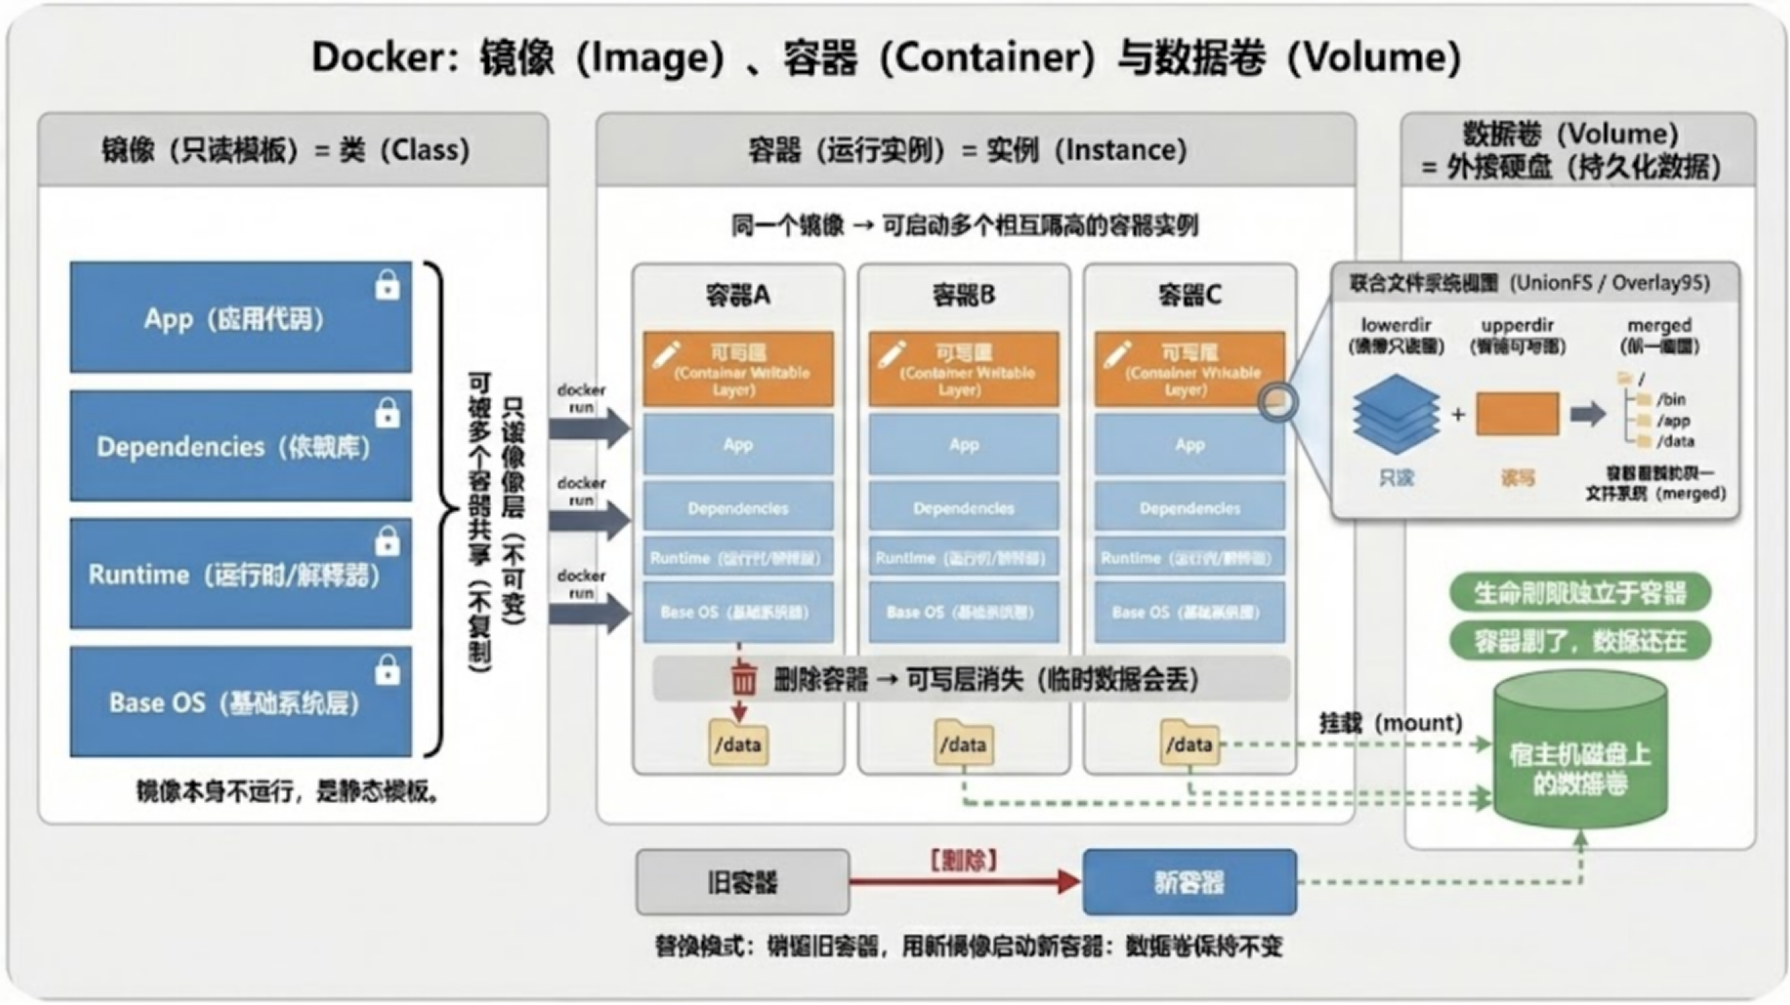
\includegraphics[width=1.0\textwidth]{figures/sec5/chapter5-2.png}
    \caption{镜像、容器以及数据卷}
    \label{fig:chapter5-2}
    \vspace{-15pt}
\end{figure*}

在Docker的概念体系中，有两个必须区分的核心概念：镜像（Image）与容器（Container）。它们的关系就是面向对象编程中"类"与"实例"的关系，或者说"程序"与"进程"的关系。

如图~\ref{fig:chapter5-2}所示，镜像是一份静态的、只读的系统快照，它完整记录了软件运行所需的一切：应用代码、依赖库、系统工具，乃至精简的操作系统用户空间。镜像一旦构建完成即不可篡改。容器则是镜像在宿主机上启动后的动态实例——一个被隔离的沙盒进程。基于同一个镜像可以启动多个容器，它们拥有独立的进程空间与网络环境，彼此隔离、互不干扰。

从系统实现的角度看，容器之所以能做到秒级启动且资源占用极低，秘密在于联合文件系统（UnionFS）的分层复用机制。观察图中容器A、B、C的内部结构：它们底部共享同一组只读的镜像层，Docker仅在其上挂载了一层薄薄的可写层。运行期间程序产生的所有状态变更——写日志、生成缓存、修改配置——都发生在这个可写层里，底下的镜像层始终保持只读。

这种设计带来一个必须警惕的副作用：可写层的生命周期与容器绑定。一旦容器被删除，可写层随之消失，其中的数据永久丢失。这就引出了一个工程问题：数据库文件、玩家存档这些需要持久保存的数据该放在哪里？

Docker的答案是数据卷（Volume）。如图~\ref{fig:chapter5-2}右侧所示，数据卷相当于一块挂载在容器上的"外接硬盘"。通过挂载操作，容器内部路径（如\texttt{/data}）被映射到宿主机磁盘上的一个目录。程序向这些路径写入数据时，数据流直接穿透可写层，落入宿主机磁盘。这样，计算逻辑（容器）与业务数据（卷）的生命周期就被彻底解耦——删除容器、升级镜像，只要挂载点不变，新容器依然能无缝接管之前的数据。

\subsubsection{隔离原理：Namespace与Cgroups}

\begin{figure*}[htbp]
    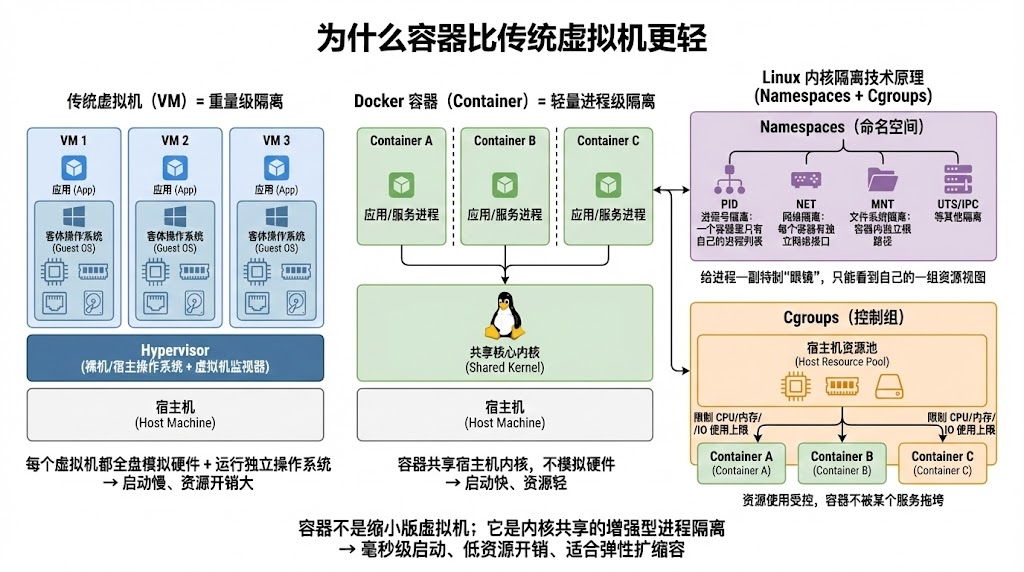
\includegraphics[width=1.0\textwidth]{figures/sec5/chapter5-3.png}
    \caption{容器与虚拟机的对比}
    \label{fig:chapter5-3}
    \vspace{-15pt}
\end{figure*}

容器能像虚拟机一样隔离运行服务，但为什么云计算普遍选择容器而非虚拟机？根本原因在于两者的隔离机制截然不同。

如图~\ref{fig:chapter5-3}左侧所示，传统虚拟机架构中每个实例都包含一套完整的Guest OS与模拟硬件层。这就像为了安顿一位客人，你得先建造一整栋独立的房子。反观图中间的容器架构，那层厚重的Guest OS彻底消失了，所有容器直接坐落在共享的宿主机内核之上。容器不需要重复启动内核，省去了漫长的开机自检与内存损耗，从而实现秒级启动与极低资源开销。

那么Docker如何让这些共享内核的进程"感觉"自己在独立运行？答案藏在图~\ref{fig:chapter5-3}右侧：Linux内核通过两大机制为进程构建隔离边界。

第一个是Namespace（命名空间）。它在PID（进程号）、NET（网络栈）、MNT（文件挂载点）等维度上为进程构建独立的视图：容器内部只能看到自己的进程列表和网络接口，完全感知不到宿主机上其他进程的存在。第二个是Cgroups（控制组）。它直接对接宿主机的资源池，严格限制每个容器能消耗的CPU时间片和内存上限，防止单个容器因资源失控而拖垮整台服务器。

理解了这两个机制，我们就能建立对容器最准确的直觉：容器不是"缩小版的虚拟机"，而是一个"自带隔离边界的增强型进程"。正是"共享内核"与"独占边界"的结合，让容器在保留隔离性的同时将资源利用率推向极致。

容器的网络隔离也依赖Namespace。Docker启动容器时，会把它放进独立的Network Namespace，容器内部看到的是自己专属的网络设备、IP地址和路由表。Docker通常为容器创建一对\texttt{veth}虚拟网卡——像一根"虚拟网线"的两端：一端放入容器的网络命名空间作为网络出口，另一端留在宿主机侧接入\texttt{docker0}网桥。同一宿主机上的多个容器通过\texttt{docker0}互联：数据包从源容器的\texttt{veth}端口进入网桥，再由网桥转发到目标容器的\texttt{veth}端口。

需要强调的是，容器与虚拟机在隔离强度上并不等价。容器共享宿主机内核，内核攻击面的隔离相对更弱；虚拟机为每个实例提供独立内核，边界更强但资源成本更高。在多租户云环境中，常见做法是引入gVisor、Kata Containers等轻量虚拟化方案，在性能与隔离之间取得折中。这些方案的原理将在第六章讨论。

\subsubsection{制作镜像：Dockerfile与分层构建}\label{sec:dockerfile}

\begin{figure*}[htbp]
    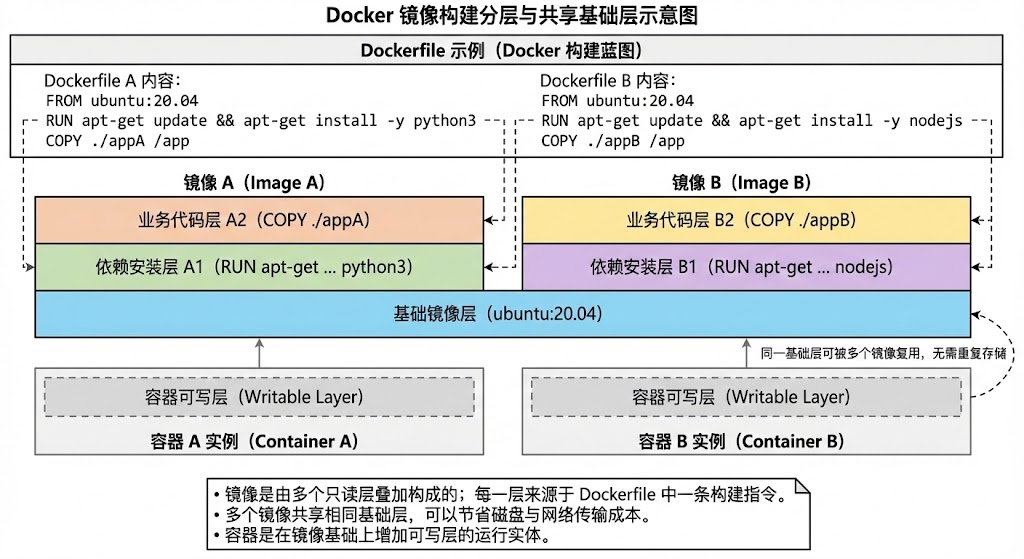
\includegraphics[width=1.0\textwidth]{figures/sec5/chapter5-1.png}
    \caption{Dockerfile构建镜像过程}
    \label{fig:chapter5-1}
    \vspace{-15pt}
\end{figure*}

镜像不是一个简单的压缩包，而是严格基于Dockerfile（构建蓝图）逐层生成的。如图~\ref{fig:chapter5-1}所示，Dockerfile中的每一行指令——无论是\texttt{FROM}定义的基础环境，还是\texttt{RUN}执行的软件安装——都会被转化为镜像中一个独立的只读层。这些层按指令顺序由下至上累积，每层仅记录相对于上一层的增量变化。

这种"指令即图层"的设计带来两个关键优势。第一是资源复用：如图中部蓝色区域所示，虽然镜像A与镜像B的上层业务代码不同，但它们共享同一个\texttt{ubuntu:20.04}基础层，物理存储上只需保存一份。部署大规模微服务时，系统仅需为各服务的差异部分"付费"，极大降低磁盘占用与网络传输成本。第二是构建缓存：Docker采用内容寻址存储（Content-Addressable Storage），每个镜像层由SHA256摘要唯一标识。只要某一层的输入没有变化，Docker就直接复用缓存而不重新构建，日常只改业务代码时通常只需重建最上面一两层。

回到我们的游戏项目。第四章中我们将后端拆分为大厅服与战斗服两个独立模块，未来还可能水平扩容（增开一区、二区）。如果为每个服务单独维护一份Dockerfile，维护成本会成倍攀升。下面这份通用Dockerfile通过构建参数实现了"一份蓝图，多个服务"的复用：

\begin{tcolorbox}[title=通用Dockerfile：多阶段构建]
\begin{lstlisting}[language=bash,basicstyle=\ttfamily\footnotesize,numbers=left,numberstyle=\tiny\color{gray},numbersep=5pt,aboveskip=0pt,belowskip=0pt,lineskip=-1pt,commentstyle=\color{gray},keywordstyle=\color{blue}\bfseries,breaklines=true,showstringspaces=false]
FROM golang:1.21-alpine AS builder
WORKDIR /app
COPY go.mod go.sum ./
RUN go mod download
COPY . .
ARG SERVICE
RUN if [ -z "$SERVICE" ]; then echo "ERR: SERVICE not set"; exit 1; fi
RUN CGO_ENABLED=0 GOOS=linux go build -o server_bin ./cmd/${SERVICE}
FROM alpine:latest
RUN apk --no-cache add ca-certificates tzdata
WORKDIR /root/
COPY --from=builder /app/server_bin .
COPY --from=builder /app/config ./config
CMD ["./server_bin"]
\end{lstlisting}
\end{tcolorbox}

这份Dockerfile的核心不在于命令语法，而在于三个工程决策。其一，多阶段构建：第一阶段（\texttt{builder}）使用包含Go工具链的完整编译环境（约300\,MB），第二阶段切换到仅5\,MB的Alpine基础镜像，只从第一阶段复制编译产物。最终镜像通常只有10--15\,MB，扩容时节点拉取镜像的时间显著缩短。其二，依赖缓存优化：先复制\texttt{go.mod}与\texttt{go.sum}并下载依赖，再复制源码。由于依赖变动频率远低于业务代码，这种顺序能最大化缓存命中率。其三，静态编译：\texttt{CGO\_ENABLED=0}生成的二进制自带所有依赖，不依赖宿主机的动态链接库，这也是容器能运行在极简环境中的前提。关于每行指令的详细解读，请参见附录~\ref{sec:appendix-dockerfile}。

\subsubsection{分发镜像：Registry与版本锁定}

\begin{figure*}[htbp]
    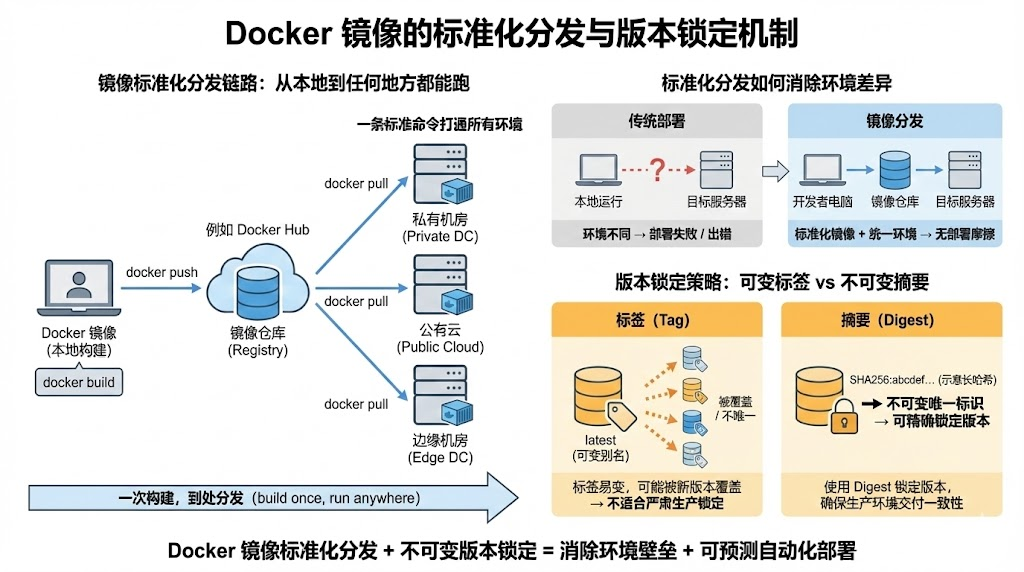
\includegraphics[width=1.0\textwidth]{figures/sec5/chapter5-4.png}
    \caption{Docker的标准化分发链路}
    \label{fig:chapter5-4}
    \vspace{-15pt}
\end{figure*}

镜像构建完成后，如何让三台云服务器都能拿到同一份镜像？Docker通过镜像仓库（Registry）机制解决这个问题。如图~\ref{fig:chapter5-4}所示，开发者用\texttt{docker push}将镜像推送到远端仓库（如Docker Hub或云厂商的私有仓库），运维人员在任意服务器上用\texttt{docker pull}即可将完整的运行环境原样拉取下来。Docker的分层机制确保只上传云端缺失的增量层，节省带宽。

在生产环境中，版本锁定是一个容易被忽视但至关重要的环节。Docker提供了\texttt{latest}等标签（Tag）机制，但标签本质上是可变的别名——今天拉取的\texttt{latest}和明天拉取的可能是完全不同的代码。因此工程实践中更倾向于使用镜像摘要（Digest），即对镜像内容进行SHA256哈希计算生成的唯一标识符。通过摘要锁定版本，可以确保无论何时何地拉取，得到的都是同一份镜像。

下面是完整的镜像发布流程：

\begin{tcolorbox}[title=镜像发布与版本锁定]
\begin{lstlisting}[language=bash,basicstyle=\ttfamily\footnotesize,numbers=left,numberstyle=\tiny\color{gray},numbersep=5pt,aboveskip=0pt,belowskip=0pt,lineskip=-1pt,commentstyle=\color{gray},keywordstyle=\color{blue}\bfseries,breaklines=true,showstringspaces=false]
docker build -t game-lobby:v1 .                        # 构建镜像
docker login                                            # 登录镜像仓库
docker tag game-lobby:v1 username/game-lobby:v1         # 打标签
docker push username/game-lobby:v1                      # 推送到云端
docker pull username/game-lobby@sha256:[digest]         # 按摘要拉取
docker images --digests                                 # 验证一致性
\end{lstlisting}
\end{tcolorbox}

至此，我们解决了单个容器的标准化交付问题：从构建、分发到版本锁定，形成了一条完整的流水线。但现实中的游戏后端不止一个服务——大厅服、战斗服、Redis、MySQL、Nginx至少五个组件需要协同启动。手动逐个\texttt{docker run}不仅繁琐，而且启动顺序、网络互联、配置传递都容易出错。下一节我们用Docker Compose来解决这个问题。


\subsection{多容器编排：用Compose一键开服}

\subsubsection{手工启动的痛苦}

回想第四章构建的分布式架构，我们至少有网关服务、战斗服务、Redis缓存和MySQL数据库四个组件。要让游戏后端运行起来，必须协调启动多个容器，并保证启动顺序、网络连接和配置传递正确无误。如果用手工方式，流程大致如下：

\begin{tcolorbox}[title=手工启动多个容器]
\begin{lstlisting}[language=bash,basicstyle=\ttfamily\footnotesize,numbers=left,numberstyle=\tiny\color{gray},numbersep=5pt,aboveskip=0pt,belowskip=0pt,lineskip=-1pt,commentstyle=\color{gray},keywordstyle=\color{blue}\bfseries,breaklines=true,showstringspaces=false]
docker run -d --name mysql-db -e MYSQL_ROOT_PASSWORD=123456 mysql
docker run -d --name redis-cache redis
docker run -d --name map-service --link mysql-db -p 8081:8080 game/map-service
docker run -d --name gateway --link map-service -p 8080:8080 game/gateway
\end{lstlisting}
\end{tcolorbox}

四个容器就需要四条命令，必须严格按顺序执行，还要手动处理端口映射和容器间链接。每次发布、每次更新都要重复这套流程，稍有疏忽就可能导致连接失败或服务不可用。

\subsubsection{Compose的声明式配置}

\begin{figure}[htbp]
\centering

\includegraphics[width=0.85\textwidth]{figures/sec5/Docker_Compose_concepts.png}
\caption{Docker Compose服务编排的核心概念与工作机制}
\label{fig:compose-concepts}
\end{figure}

Docker Compose通过一份YAML格式的声明式配置文件，将上述所有手工操作收敛为一条命令：\texttt{docker-compose up -d}。如图~\ref{fig:compose-concepts}所示，配置文件清晰描述了所有服务的镜像、端口映射、环境变量、依赖关系和网络设置。

\begin{tcolorbox}[title=Docker Compose配置示例]
\begin{lstlisting}[language=bash,basicstyle=\ttfamily\footnotesize,numbers=left,numberstyle=\tiny\color{gray},numbersep=5pt,aboveskip=0pt,belowskip=0pt,lineskip=-1pt,commentstyle=\color{gray},keywordstyle=\color{blue}\bfseries,breaklines=true,showstringspaces=false]
version: "3"
services:
  mysql-db:
    image: mysql:5.7
    environment:
      MYSQL_ROOT_PASSWORD: "123456"
    ports:
      - "3306:3306"
    volumes:
      - db-data:/var/lib/mysql
  redis-cache:
    image: redis:6
    ports:
      - "6379:6379"
  map-service:
    image: game/map-service:v1
    depends_on:
      - mysql-db
      - redis-cache
    ports:
      - "8081:8080"
    environment:
      DB_HOST: mysql-db
      REDIS_HOST: redis-cache
  gateway-service:
    image: game/gateway:v1
    depends_on:
      - map-service
    ports:
      - "8080:8080"
    environment:
      MAP_SERVICE_HOST: map-service
volumes:
  db-data:
\end{lstlisting}
\end{tcolorbox}

执行\texttt{docker-compose up}时，Compose首先解析配置文件并验证语法，然后根据\texttt{depends\_on}字段构建服务间的依赖关系图（一个有向无环图），对其进行拓扑排序以确定启动顺序。接着Compose创建一个专属的虚拟网络，并为每个服务配置DNS解析——在这个网络中，容器可以直接通过服务名（如\texttt{mysql-db}）访问其他容器，无需知道具体IP地址。最后按拓扑顺序逐个启动容器，自动完成镜像拉取、环境变量注入、端口映射和网络接入。

\begin{figure}[htbp]
\centering
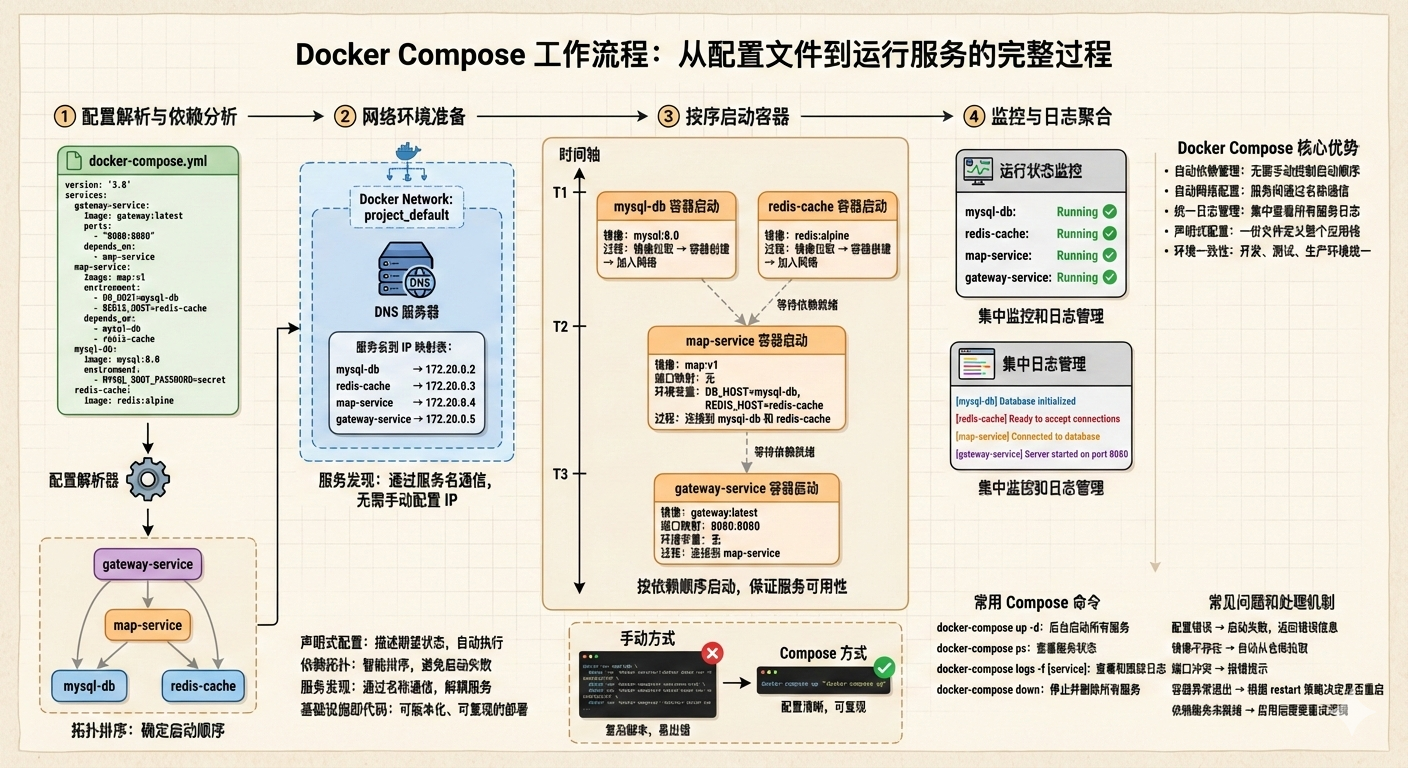
\includegraphics[width=0.9\textwidth]{figures/sec5/docker-compose-workflow.png}
\caption{Docker Compose工作流程：从配置文件到运行服务}
\label{fig:compose-workflow}
\end{figure}

这里有两个细节值得注意。第一，\texttt{depends\_on}只保证容器的启动顺序，不等待服务真正就绪。例如MySQL容器已经启动，但数据库服务本身可能还在初始化，尚未准备好接受连接。应用代码需要实现重试逻辑来应对这种情况。第二，Compose的声明式配置天然具备幂等性：反复执行\texttt{docker-compose up}时，Compose会比对当前状态与配置文件的期望状态，只进行必要的创建或重建操作，不会产生重复容器或端口冲突。

对于需要长期运行的游戏服务，Compose还提供了重启策略：\texttt{restart: always}表示无论何种退出都自动拉起，\texttt{on-failure}只在非零退出码时重启，\texttt{unless-stopped}则尊重人工停机操作。这些策略虽然简单，却已经体现出自愈机制的雏形。

\subsubsection{Compose的边界：为什么单机编排不够}

当项目从几百名在线玩家增长到上千甚至更多时，Compose的局限性会迅速显现。它本质上依赖单一Docker Engine，所有容器集中在一台机器上运行。这意味着：一旦主机硬件故障，服务整体不可用；缺乏跨节点调度能力，无法把负载分散到多台服务器；不具备滚动更新机制，版本发布时容易引入可感知中断；没有面向实时负载的自动伸缩控制，难以应对突发流量。

这些限制并非Compose的设计缺陷——它本来就是为单机开发和测试场景设计的。当我们需要跨多台机器调度容器、自动故障恢复、滚动发布和弹性伸缩时，就需要一个真正的集群编排系统。这正是Kubernetes要解决的问题。

\subsection{Kubernetes：集群级的自动化编排}

\subsubsection{从Compose到K8s：新的问题域}

Compose解决了单机上多容器的协同启动问题，但当我们把视野从一台机器扩展到十台、五十台时，一组全新的问题浮出水面。

第一，调度问题：新启动的容器应该放在哪台机器上？需要综合考虑各节点的剩余CPU、内存、网络带宽，以及容器之间的亲和性约束。第二，故障恢复：某台服务器宕机后，上面运行的容器怎么办？需要自动在其他健康节点上重新启动。第三，滚动更新：发布新版本时，如何做到不中断服务？需要逐步替换旧容器，确保任何时刻都有足够的实例在处理请求。第四，服务发现：容器的IP地址随时可能因为重启或迁移而变化，其他服务如何找到它？

这四个问题的共同特征是：它们都超出了单机的范畴，需要一个拥有全局视野的"指挥中心"来统一协调。Kubernetes（简称K8s）正是这样一个系统。

\subsubsection{核心概念：Pod、Deployment、Service}

\begin{figure}[htbp]
\centering
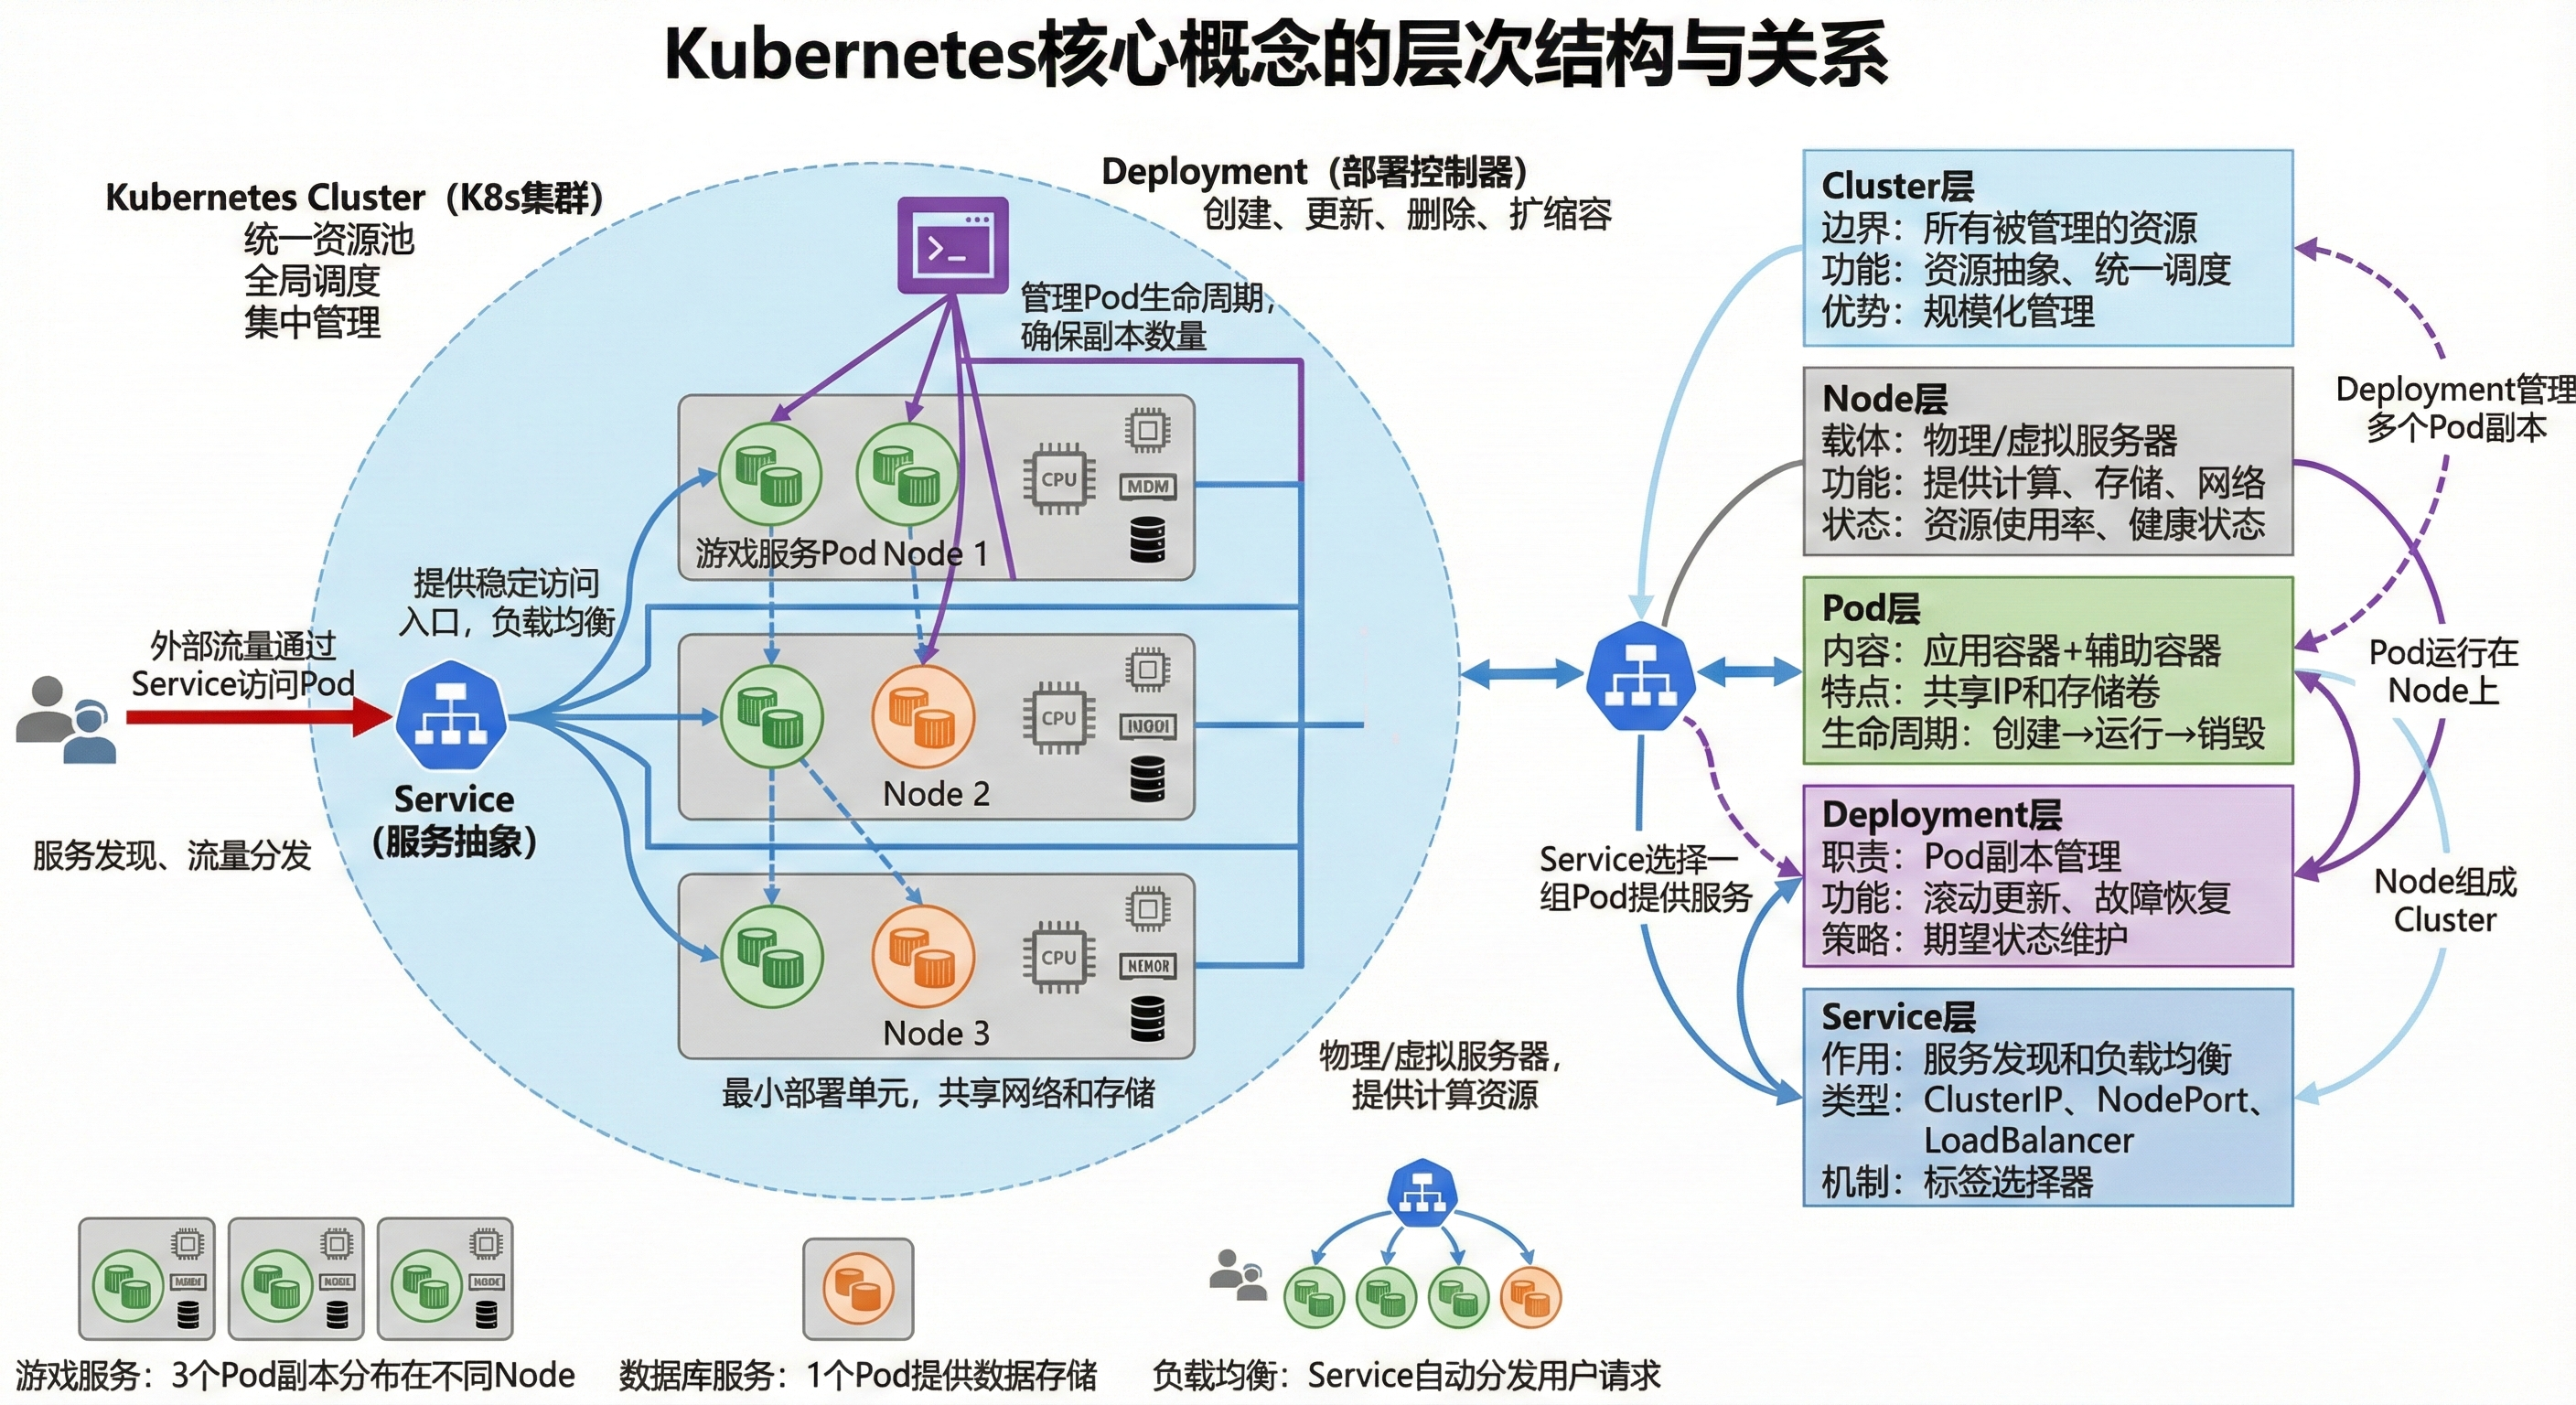
\includegraphics[width=0.9\textwidth]{figures/sec5/kubernetes-architecture-concepts.png}
\caption{Kubernetes核心概念的层次结构与关系}
\label{fig:k8s-concepts}
\end{figure}

Kubernetes的概念体系可以从底向上理解。如图~\ref{fig:k8s-concepts}所示：

\textbf{Node}（节点）是集群中的一台物理服务器或云主机，提供CPU、内存和网络等计算资源。\textbf{Pod}是K8s中最小的部署单元，通常包含一个主应用容器和可选的辅助容器（如日志收集），它们共享网络和存储，必须调度到同一个Node上运行。\textbf{Deployment}负责管理Pod的生命周期——确保始终有期望数量的Pod在健康运行，某个Pod故障时自动创建替代品，版本更新时协调滚动替换。\textbf{Service}为一组功能相同的Pod提供统一的访问入口和负载分发，外部请求通过Service到达后端Pod，无需知道具体哪个Pod在处理。

这套概念与第四章的架构有直接的对应关系。第四章中我们手工维护Nginx的\texttt{upstream}列表来实现负载均衡，每次后端实例变化都要改写配置并执行\texttt{nginx -s reload}。在K8s中，Service基于Pod的标签（Label）持续观察成员变化，由kube-proxy组件自动刷新端点列表——不再需要手动维护服务器清单。第四章的协调服务器负责服务注册与发现，在K8s中这个职责下沉为基础设施能力：CoreDNS为每个Service自动生成域名（如\texttt{game-server.default.svc.cluster.local}），集群内任何Pod都可以通过域名直接访问其他服务。

下面是一个完整的K8s配置示例，定义了一个运行三个副本的游戏服务及其负载均衡入口：

\begin{tcolorbox}[title=Kubernetes部署配置]
\begin{lstlisting}[language=bash,basicstyle=\ttfamily\footnotesize,numbers=left,numberstyle=\tiny\color{gray},numbersep=5pt,aboveskip=0pt,belowskip=0pt,lineskip=-1pt,commentstyle=\color{gray},keywordstyle=\color{blue}\bfseries,breaklines=true,showstringspaces=false]
apiVersion: apps/v1
kind: Deployment
metadata:
  name: game-server
spec:
  replicas: 3
  selector:
    matchLabels:
      app: game
  template:
    metadata:
      labels:
        app: game
    spec:
      containers:
      - name: game-server
        image: game/server:v1
        ports:
        - containerPort: 8080
        resources:
          requests:
            memory: "512Mi"
          limits:
            memory: "1Gi"
---
apiVersion: v1
kind: Service
metadata:
  name: game-service
spec:
  selector:
    app: game
  ports:
  - protocol: TCP
    port: 80
    targetPort: 8080
  type: LoadBalancer
\end{lstlisting}
\end{tcolorbox}

一条命令\texttt{kubectl apply -f deployment.yaml}，K8s就会自动完成调度、部署、负载均衡和健康检查。这份配置的关键在于它是声明式的：我们描述的是"期望状态"（3个副本、每个512Mi内存），而非"执行步骤"。

\subsubsection{声明式管理与Reconciliation Loop}

\begin{figure}[htbp]
\centering
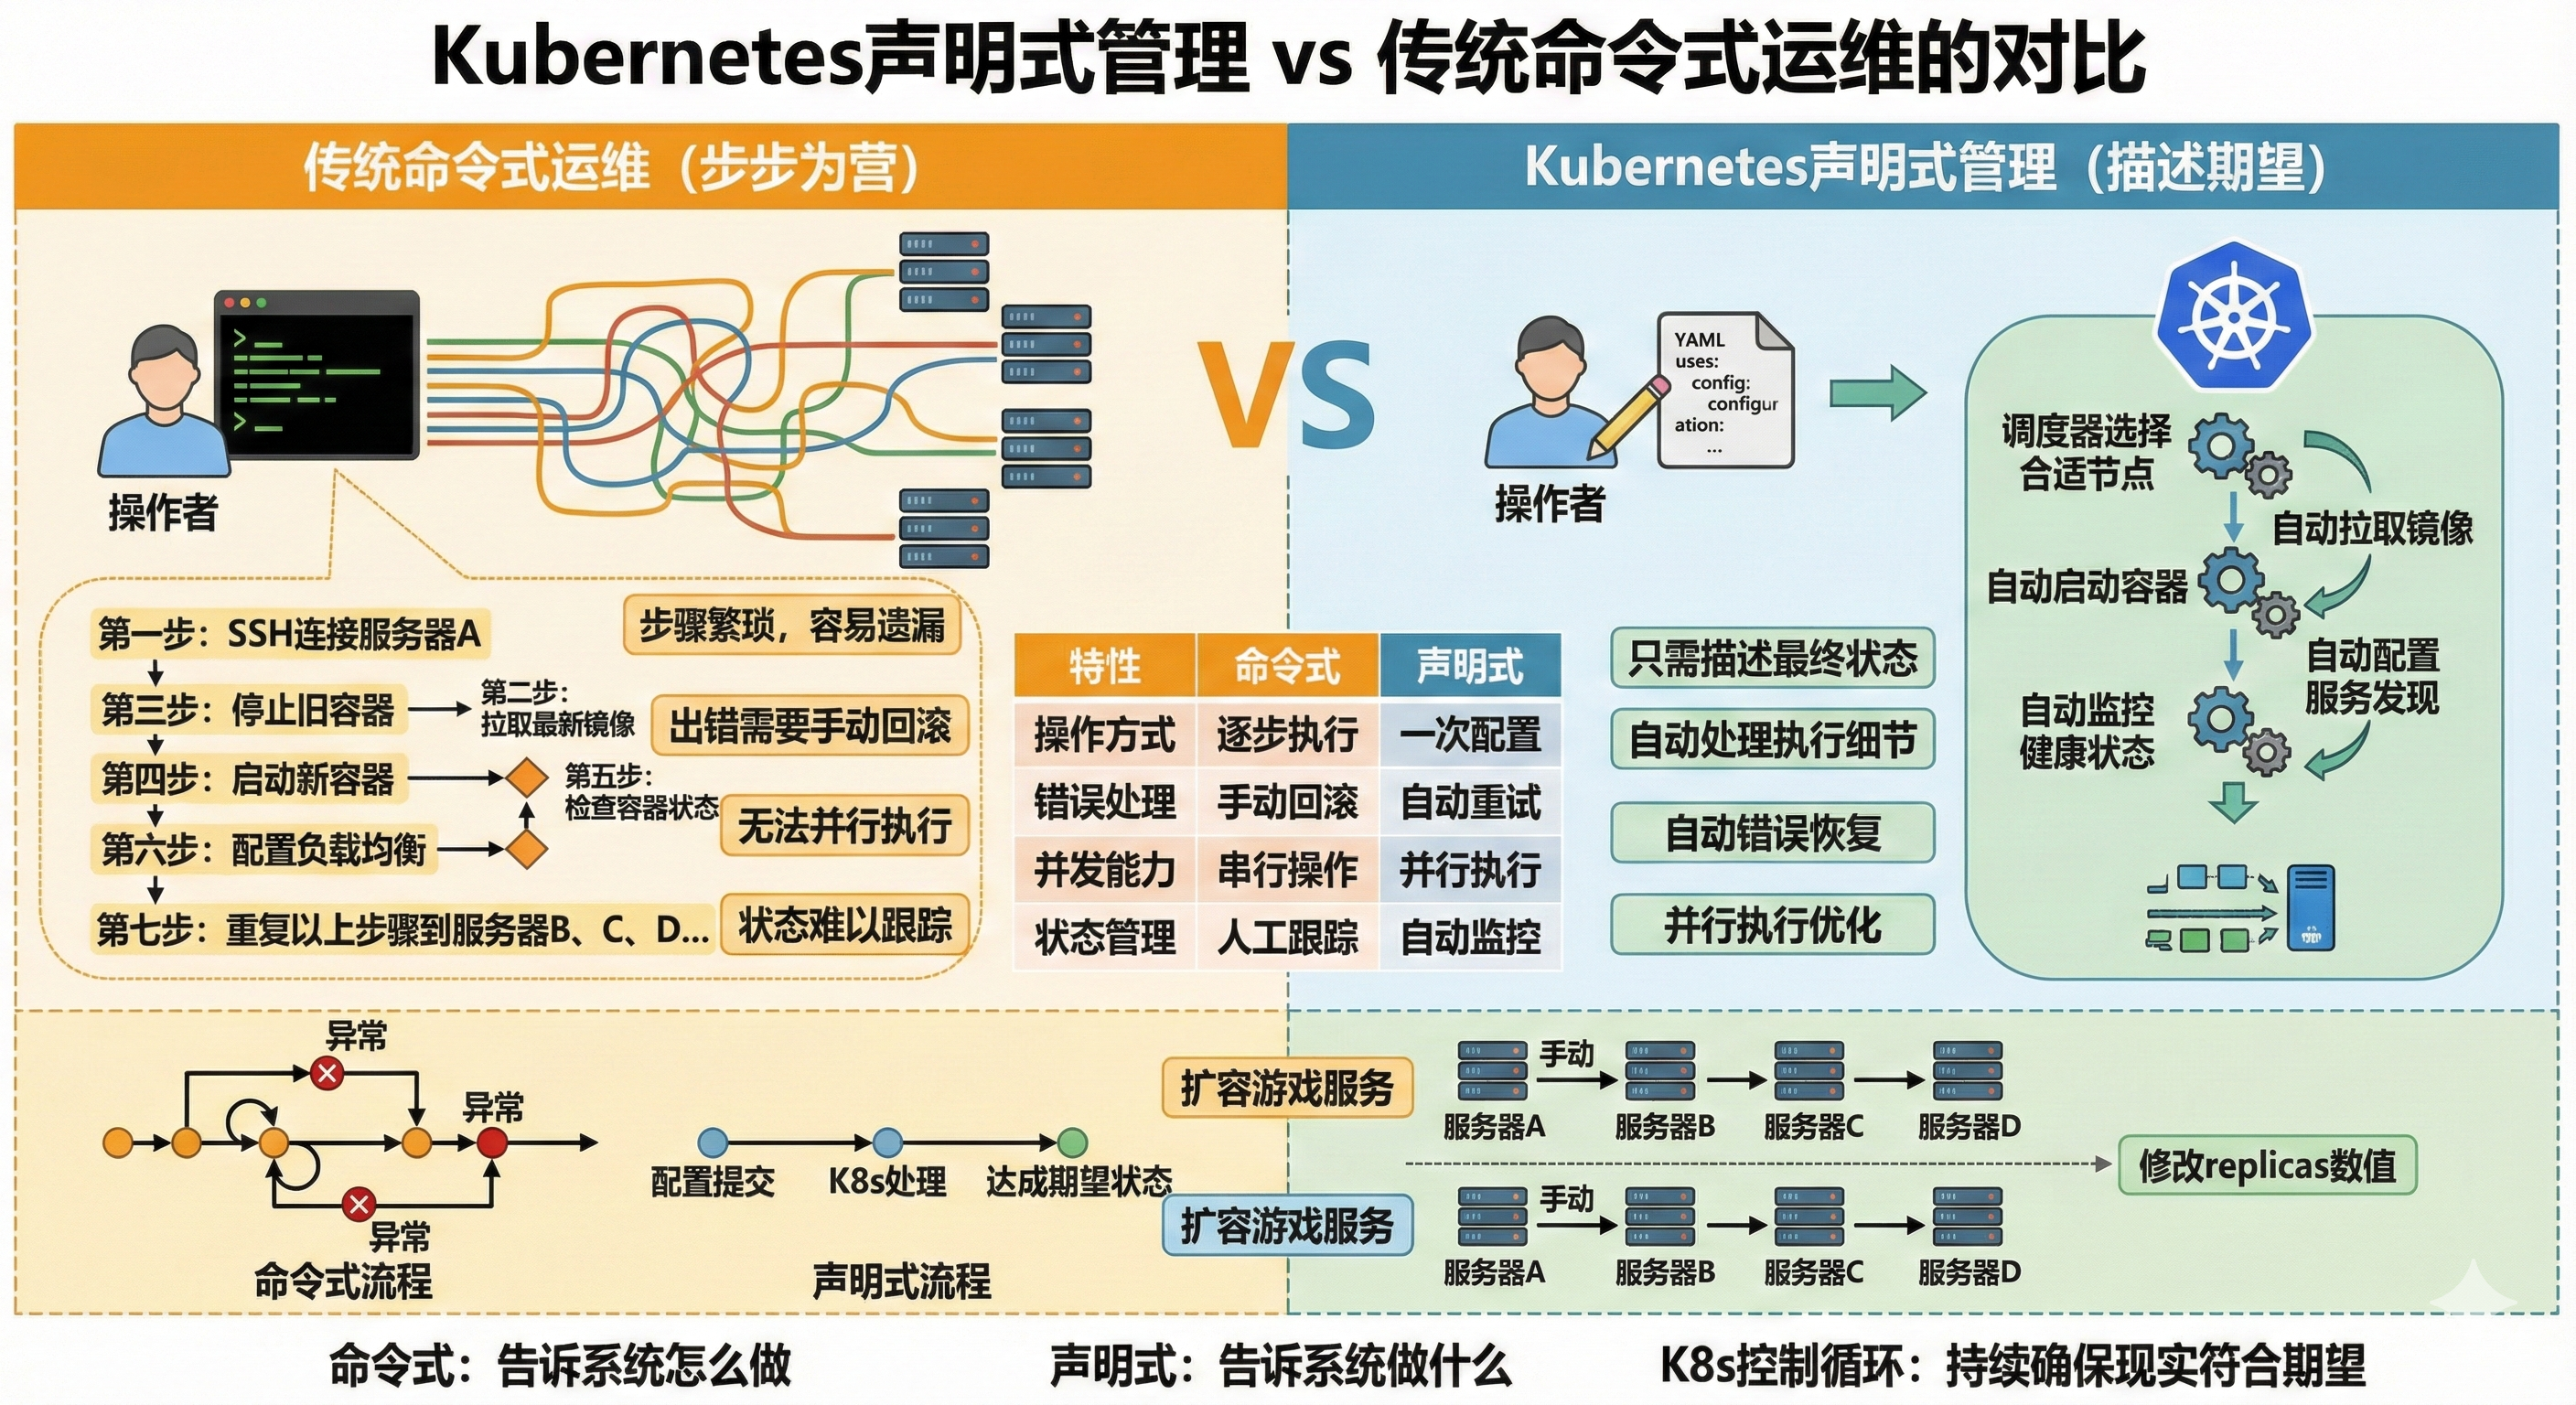
\includegraphics[width=0.9\textwidth]{figures/sec5/kubernetes-declarative-vs-imperative.png}
\caption{声明式管理与命令式运维的对比}
\label{fig:declarative-vs-imperative}
\end{figure}

声明式管理是K8s最核心的设计哲学。如图~\ref{fig:declarative-vs-imperative}所示，传统的命令式运维要求你明确指定每一个执行步骤："在服务器A上启动容器X，在服务器B上启动容器Y，配置负载均衡器指向这两个容器"。而K8s的声明式方式只需描述期望的最终状态："我需要3个游戏服务器副本在运行"，系统自动分析当前状态与期望状态的差异并执行必要操作。

这种设计的关键不在于"一次下发命令"，而在于持续运行的Reconciliation Loop（调谐循环）。控制器不断执行"观察现状、对比期望、采取动作、再次观察"的闭环，使系统逐步逼近期望状态。这属于Level-triggered思路——关注的是"现在是否达标"，而非"刚刚发生了什么事件"。即便某次消息丢失或某个操作失败，下一轮循环仍会重新发现偏差并自动修正。系统的鲁棒性来自反复校准，而非假设每条通知都可靠送达。

用游戏场景来讲：运营者只需声明"城门始终保持3名守卫"，某个守卫倒下后，控制逻辑会在后续轮次自动补位，而不需要人工逐条下达替补指令。当你需要扩容时，只需把"3"改成"10"，K8s会自动启动7个新Pod；当你需要更新版本时，只需修改镜像标签，K8s会自动执行滚动更新，逐步替换旧Pod，确保服务不中断。

\subsubsection{调度与健康检查}

当一个新Pod需要启动时，K8s的调度器负责决定它应该运行在哪个Node上。调度过程分为两个阶段：先做过滤（Filter），根据资源请求、亲和与反亲和规则、污点容忍等约束剔除不合适的Node；再做打分（Score），对候选Node按剩余资源、负载均衡度等指标评分排序，选择当前最优者。

从理论上看，这本质上是一个多维资源装箱问题——CPU、内存、带宽与拓扑同时参与决策，计算复杂性通常被视为NP-hard，因此工程实现强调近似最优与可扩展性。其思想脉络可追溯到Google的Borg系统，随后发展到Omega，再到今天的Kubernetes。用游戏比喻：调度器像在给玩家分配房间，不只看空位多少，还要兼顾延迟、容量与地域。

Pod启动后，K8s通过探针（Probe）机制持续监控其健康状态。还记得第四章中我们为游戏服务器实现的健康检查端点吗？协调服务器定期发送HTTP请求，连续几次无响应就将其从可用列表中移除。K8s采用同样的思路，但拆分为两类探针：\textbf{Liveness Probe}检测进程是否"活着但已失效"（如死锁），触发容器重启；\textbf{Readiness Probe}检测实例是否已准备好接收流量，未就绪时将其临时移出Service的负载均衡池。核心思想不变，只是由平台统一执行，而非业务代码重复实现。

\begin{figure}[htbp]
\centering
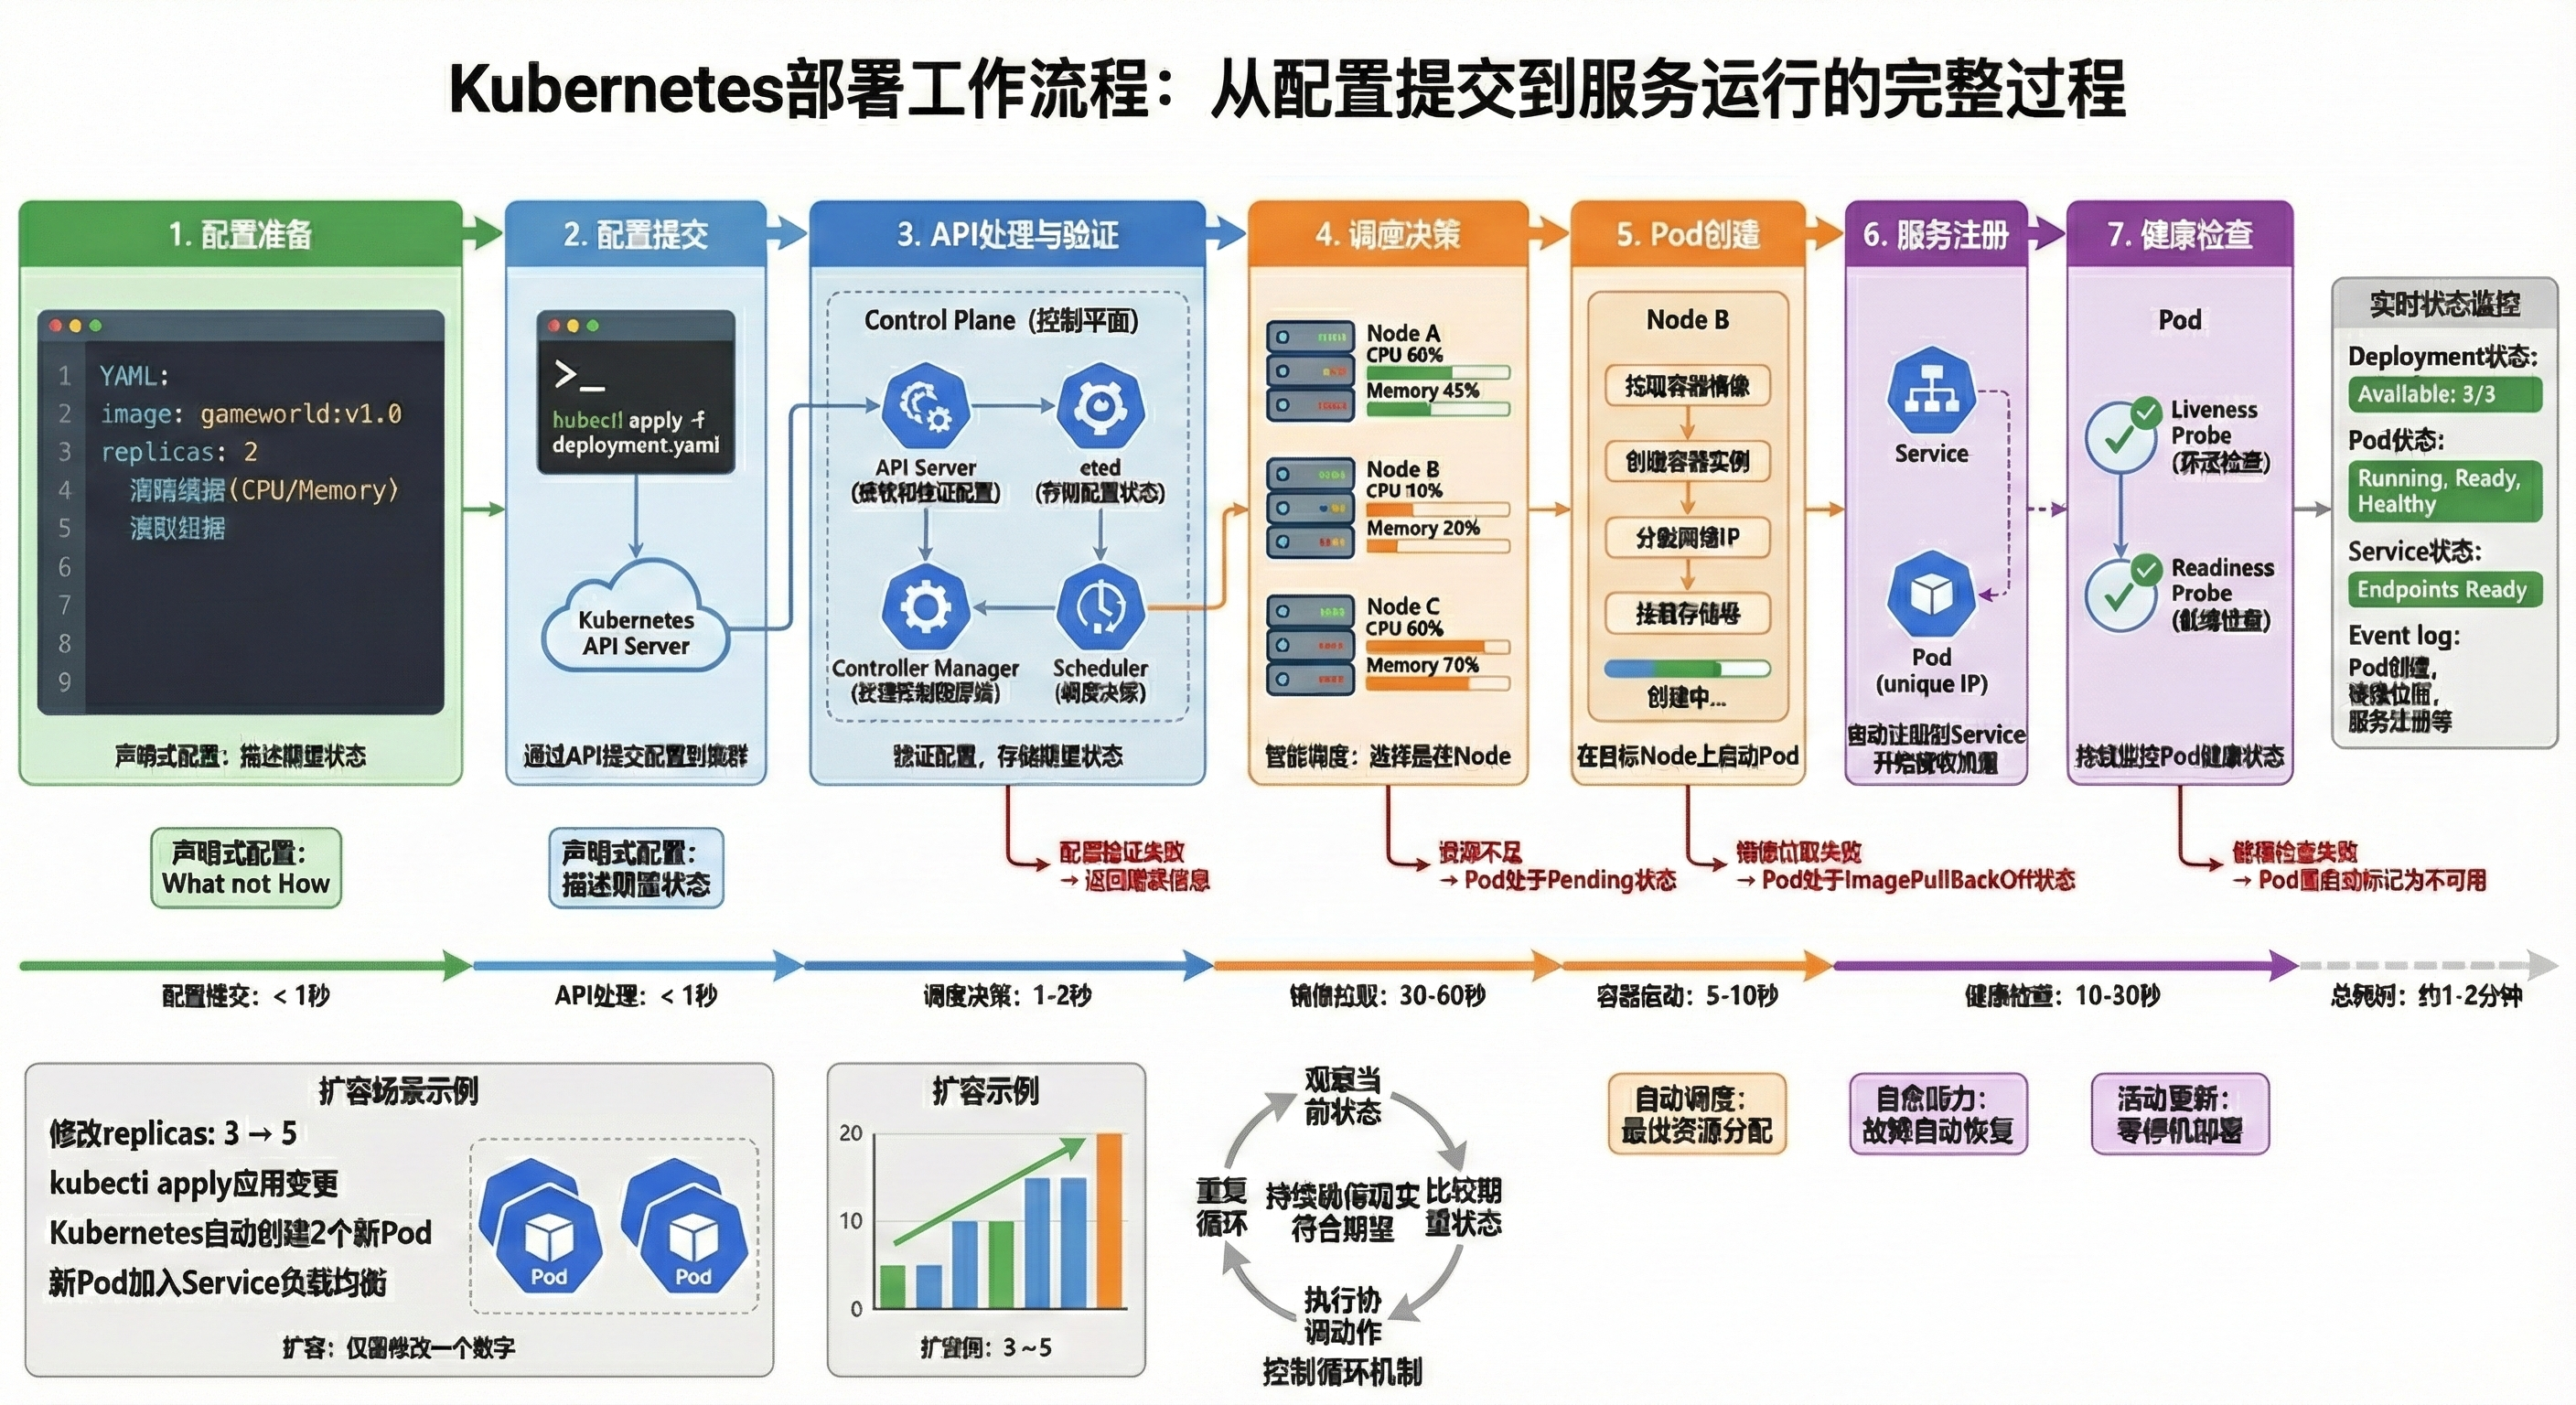
\includegraphics[width=0.9\textwidth]{figures/sec5/kubernetes-deployment-workflow.png}
\caption{Kubernetes部署工作流程：从配置提交到服务运行}
\label{fig:k8s-workflow}
\end{figure}

如图~\ref{fig:k8s-workflow}所示，从配置提交到服务稳定运行，整个过程是高度自动化的闭环：调度器选择Node，kubelet启动容器，探针监控健康状态，Service自动更新端点列表。当某个Pod异常退出时，Deployment控制器立即启动替代Pod，调度器为其选择合适的Node，整个恢复过程无需人工干预。

理解了上述核心概念后，读者可以参照附录~\ref{sec:appendix-k8s-deploy}的实战指南，亲手完成从编写YAML配置、执行\texttt{kubectl apply}到监控部署状态的完整流程。

\subsubsection{游戏服务的特殊挑战}

在将游戏后端迁移到K8s的过程中，有几个游戏场景特有的问题值得专门讨论。

第一个是协议选择。实时战斗场景对延迟和抖动极为敏感，核心链路通常选用UDP以避免TCP的队头阻塞。K8s的Service对UDP是原生支持的，端口声明后即可进行四层转发与负载分担。但需要注意，常见的Nginx Ingress主要工作在HTTP/HTTPS语义层，默认不能直接代理通用UDP流量。生产环境中更稳妥的做法是为游戏服单独创建\texttt{type: LoadBalancer}的Service，由云厂商的负载均衡器直接暴露UDP四层入口。这里要区分L4与L7负载均衡：前者按传输层五元组转发，后者理解应用层协议与路由规则。游戏业务在网关设计时应先确定协议边界，再决定在哪一层实施流量治理。

第二个是有状态问题。Deployment的设计假设是无状态工作负载——任何Pod都可以被随时替换。这对大多数Web服务很合适，但游戏服务端往往在内存中维护玩家会话：第三章连接池模型里保存的连接上下文、匹配状态与短期战斗数据，都绑定在当前进程上。工程上常见两条路：

其一，将会话状态外置到Redis等外部存储，让业务Pod回到可替换的无状态形态。这更符合云原生的弹性与故障恢复思路，但每次读写状态都引入额外的网络时延与一致性成本。其二，采用StatefulSet为Pod提供稳定的网络标识与持久命名，配合Session Affinity将特定玩家的流量固定到特定Pod。这更接近传统游戏分区服架构，迁移门槛低，但会牺牲调度自由度与横向伸缩效率。

两种方案各有适用场景，没有绝对的优劣。对于登录、匹配等无状态服务，状态外置是自然选择；对于需要将玩家"粘"在特定战斗实例上的有状态场景，StatefulSet加会话亲和更为务实。这两类方案的容量评估与故障演练方法将在第六章进一步展开。

\subsection{弹性伸缩：让资源跟着玩家走}

在第四章中，当玩家负载增加时，我们的应对方式是：手动开通新的云服务器，部署游戏服务，向协调服务器注册，再修改Nginx配置。负载下降需要缩容时更加麻烦：必须先迁移玩家、确认没有活跃会话后才能安全关闭。扩缩容的每一步都需要人工操作和业务逻辑配合。

在K8s的世界里，思路完全不同：你只需声明"我希望CPU使用率保持在70\%以下"，平台就会自动增减Pod实例，Service自动调整流量分发。扩缩容从"人工操作服务器"变成了"声明期望状态"。

\subsubsection{问题：固定配置遇上波动流量}

\begin{figure}[htbp]
\centering
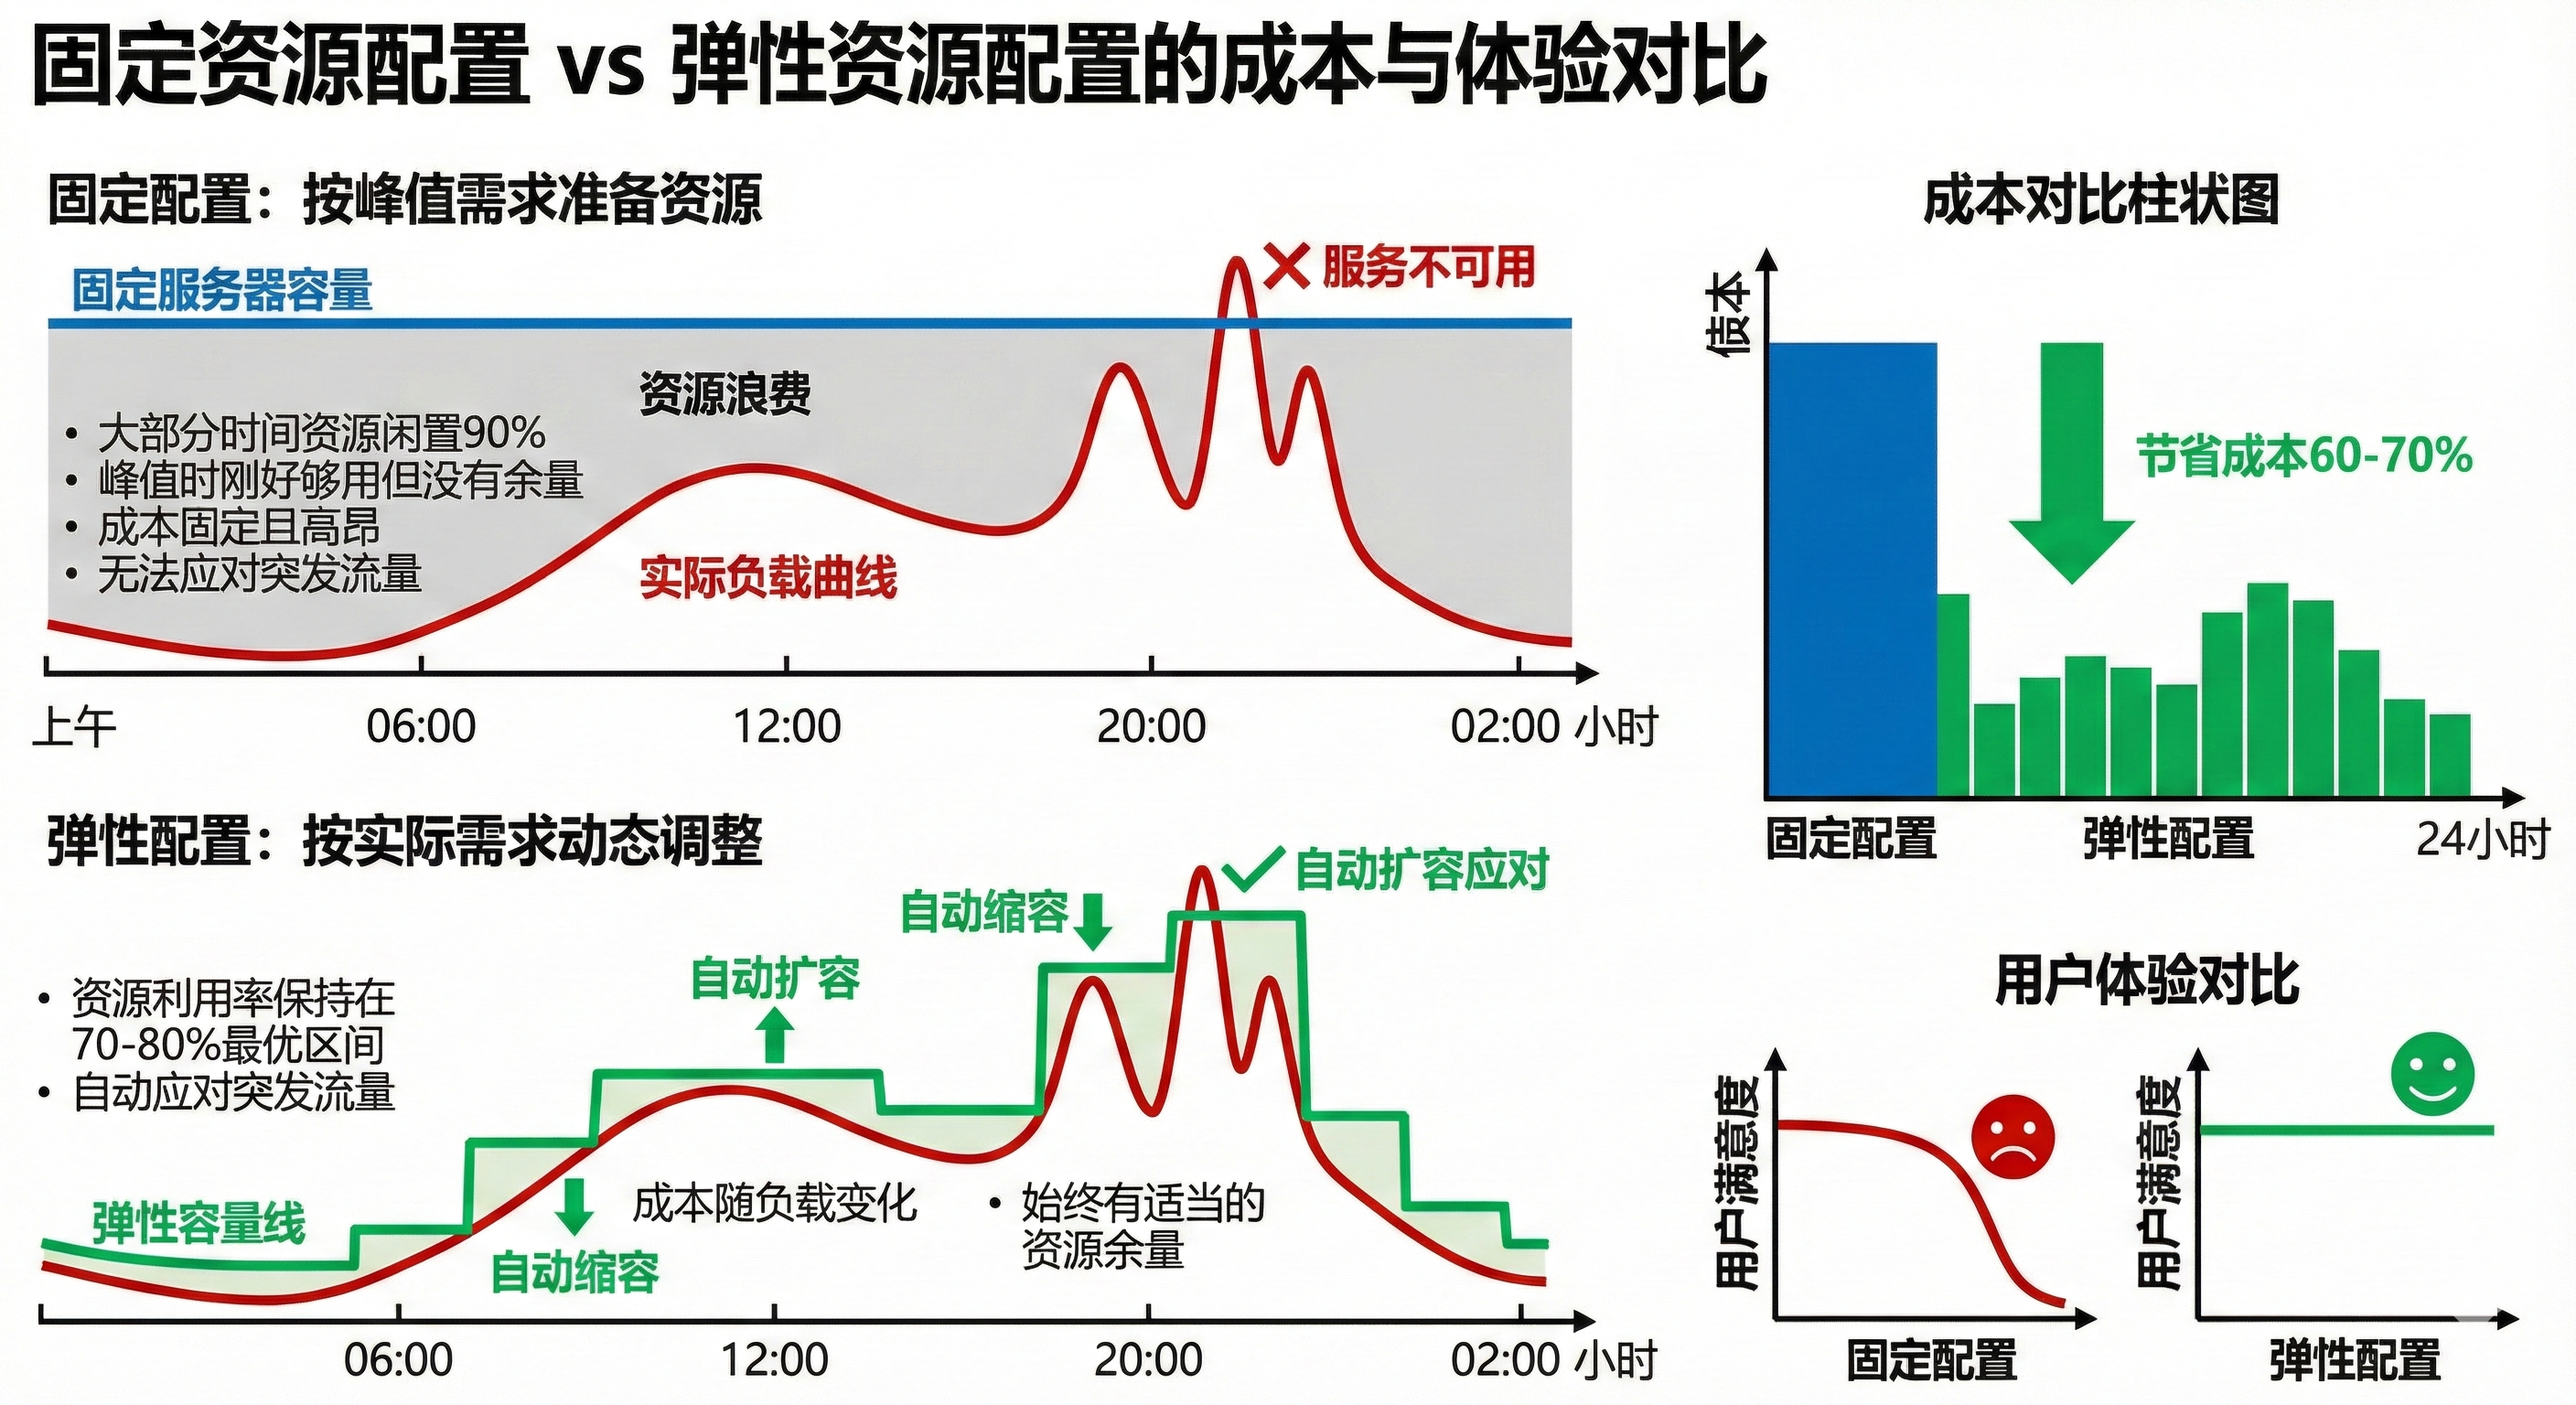
\includegraphics[width=0.9\textwidth]{figures/sec5/fixed-vs-elastic-resources.png}
\caption{固定资源配置与弹性资源配置的成本与体验对比}
\label{fig:fixed-vs-elastic}
\end{figure}

传统部署模式按业务高峰期配置服务器数量。如图~\ref{fig:fixed-vs-elastic}所示，这种策略面临结构性矛盾：周五晚上8点同时在线5万人，需要50台服务器；周二上午10点在线5000人，5台就够了。如果始终维持50台，90\%的时间里大部分资源在空转；如果按平均流量配置，高峰期就会出现连接超时和操作卡顿。

更棘手的是突发流量：一个主播的推荐、一次版本更新的热度，都可能在几分钟内让负载暴增数十倍。静态配置无法应对这种不可预测的波动。

\subsubsection{HPA：Pod级自动扩缩}

\begin{figure}[htbp]
\centering
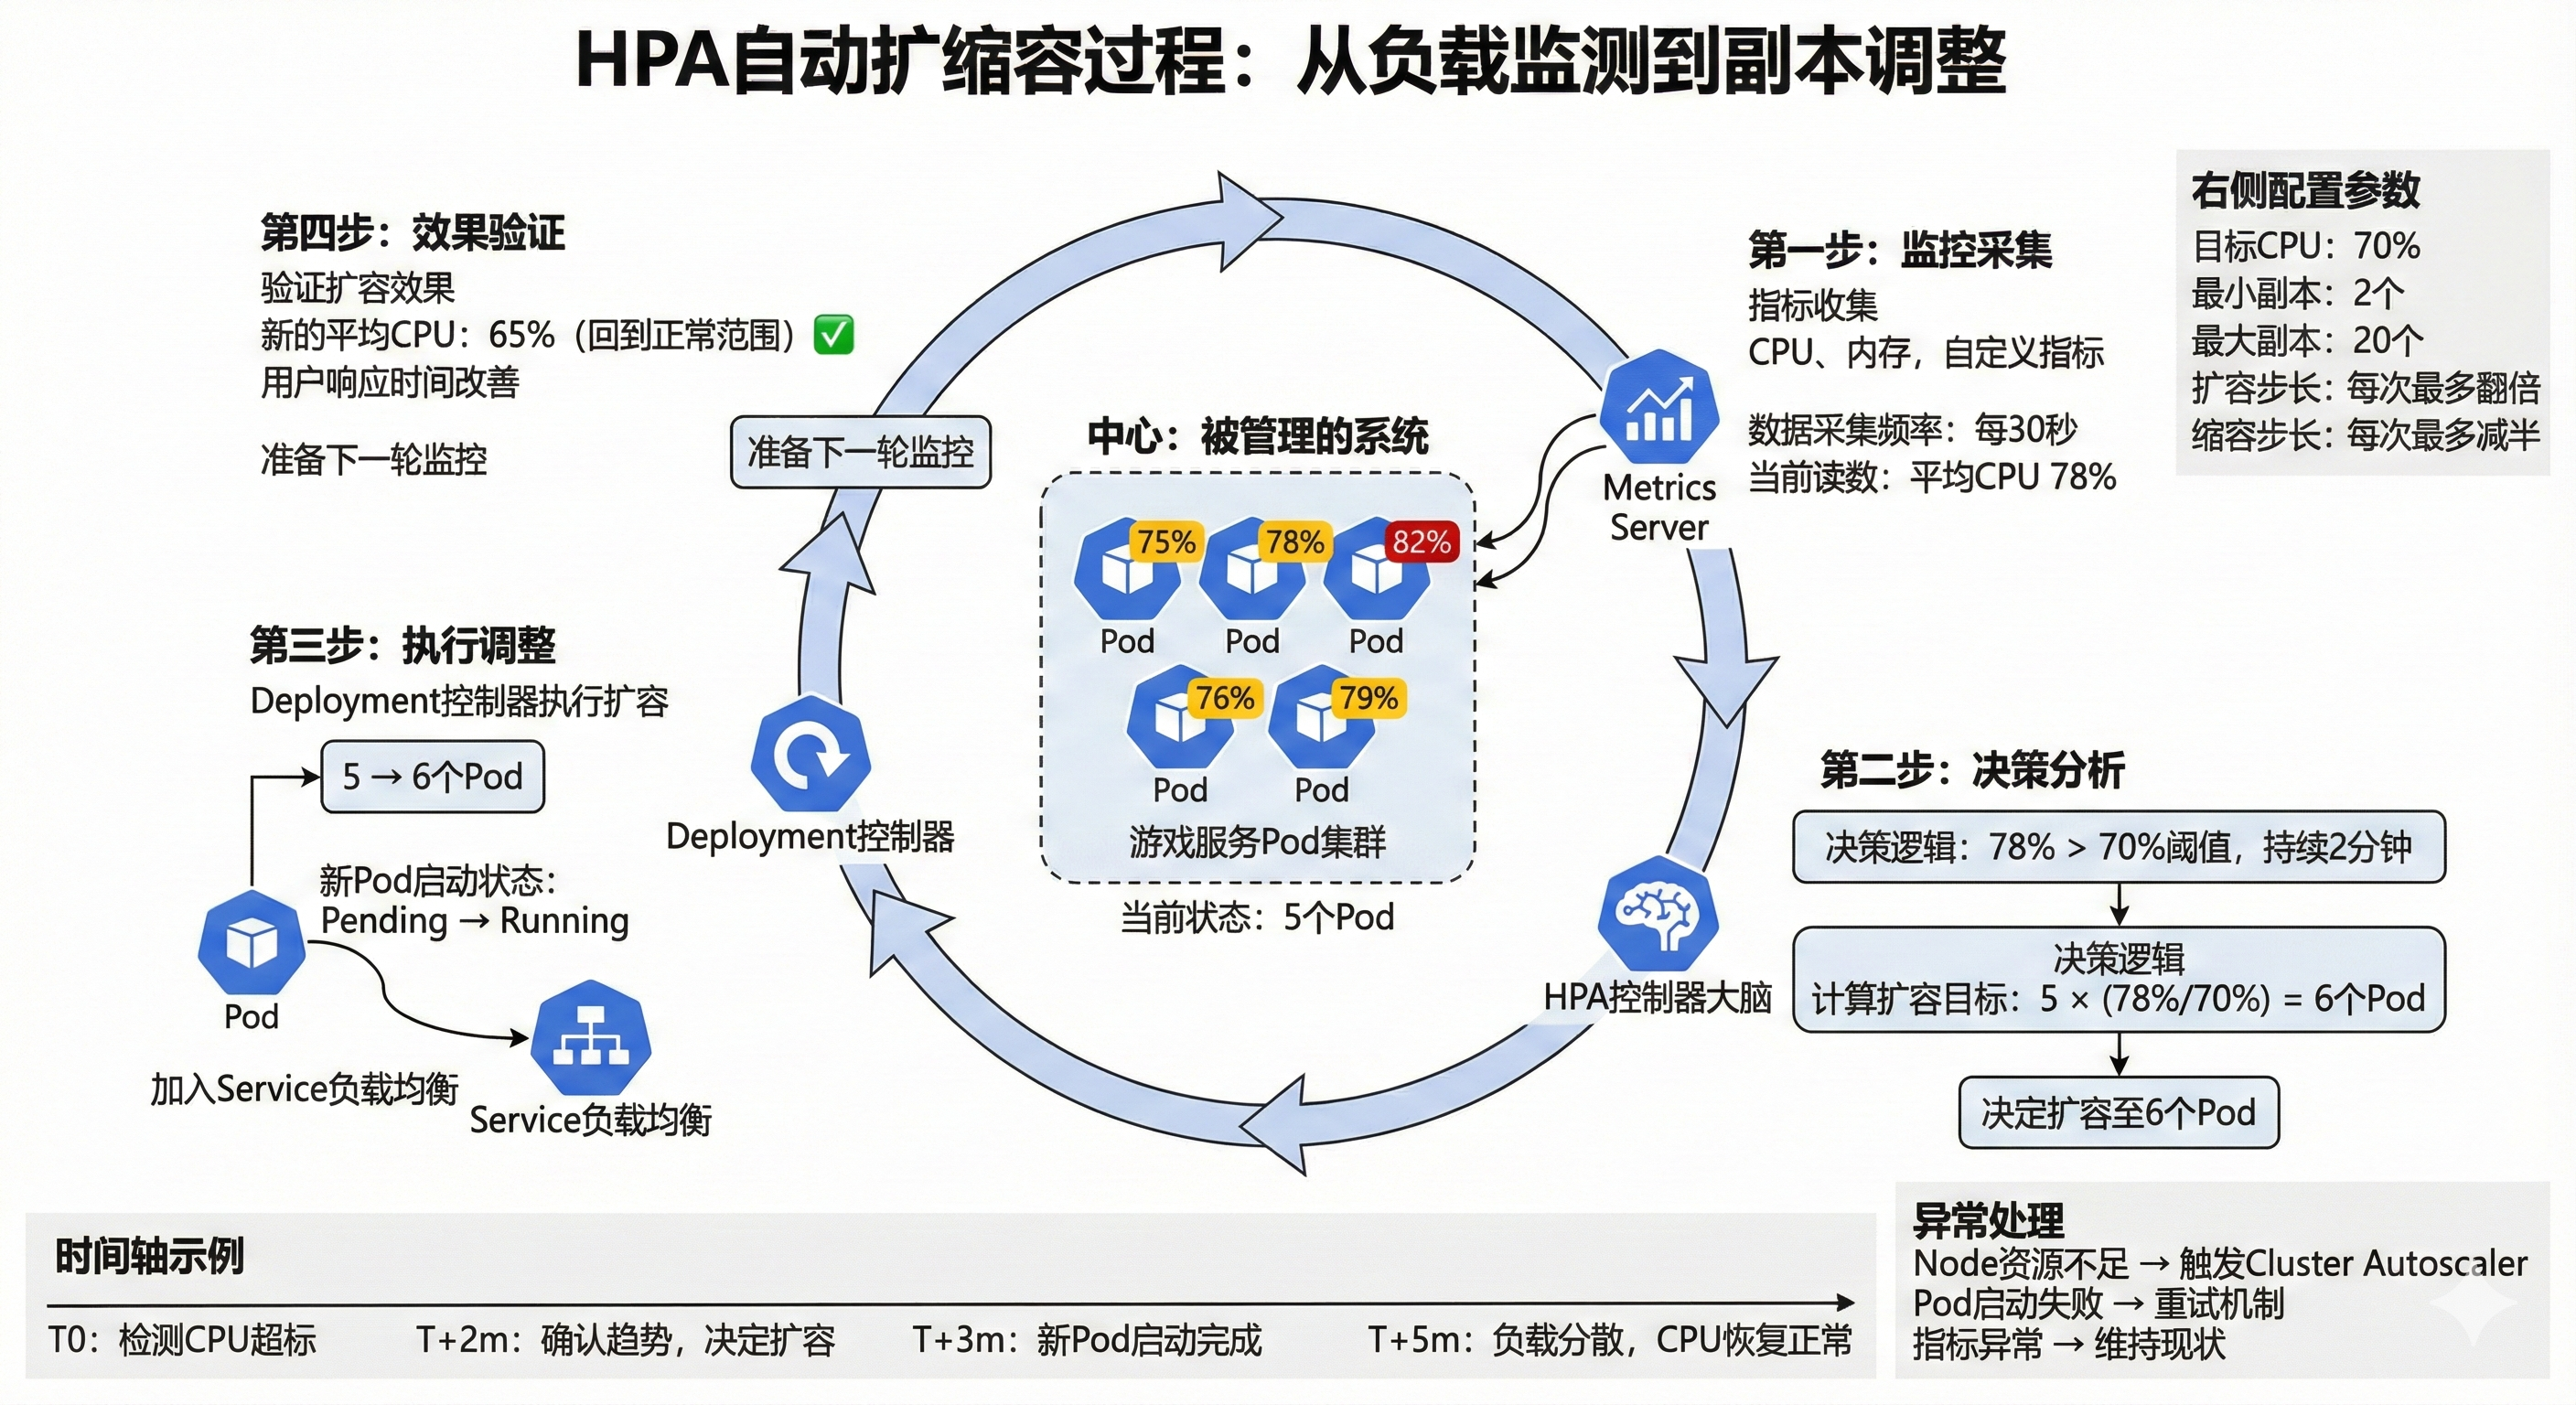
\includegraphics[width=0.9\textwidth]{figures/sec5/hpa-scaling-process.png}
\caption{HPA自动扩缩容过程：从负载监测到副本调整}
\label{fig:hpa-scaling}
\end{figure}

Horizontal Pod Autoscaler（HPA）是K8s提供的Pod级弹性方案。如图~\ref{fig:hpa-scaling}所示，HPA通过metrics server持续收集Pod的资源使用指标，当CPU使用率超过设定阈值时向Deployment发出扩容指令，负载回落时触发缩容。

从控制理论的视角看，HPA本质上是一个比例控制器（P-controller），其计算关系为：
\[
\texttt{desiredReplicas}=\lceil \texttt{currentReplicas}\times \texttt{currentMetric}/\texttt{targetMetric}\rceil
\]
例如目标CPU使用率为70\%，当前达到140\%且现有3个副本时，$\lceil 3\times 140/70\rceil=6$，扩容到6个副本。这种机制只有P项没有I项和D项，实现简单但容易出现稳态误差与振荡。为降低抖动，HPA默认设置约10\%的容忍区间，小幅偏差不触发动作，同时通过stabilization window（默认缩容5分钟、扩容0秒）防止频繁波动。

然而HPA存在固有局限。其一，端到端响应延迟：约15秒的采样周期叠加Pod启动时间，最短响应通常在45秒量级，本质上是被动响应而非提前预测。其二，热点稀释：HPA基于所有Pod的平均指标决策，如果只有个别实例因热点玩家集中而过载，平均值可能仍在阈值内，导致扩容不被触发。其三，缩容风险：对于承载活跃游戏会话的Pod，直接终止会导致玩家在对局中被强制断开。\texttt{terminationGracePeriodSeconds}为Pod预留优雅退出窗口，但这是硬超时——如果一局游戏持续20分钟而宽限期只有30秒，Pod仍会被强制终止。更务实的做法是在PreStop阶段触发"停止接收新对局"的排水状态，让当前对局自然结束，同时配合\texttt{PodDisruptionBudget}约束中断期间的最小可用副本数。

更先进的PID控制器和预测式扩缩容方案将在第六章讨论。

\subsubsection{Cluster Autoscaler：Node级扩缩}

当Pod级扩容达到Node资源的物理上限时——所有现有节点的CPU和内存都已分配完毕，新Pod处于Pending状态无法调度——就需要Node级扩容。

Cluster Autoscaler监控到Pending Pod后，分析其资源需求，请求云厂商API创建合适规格的新虚拟机实例。新Node启动并加入集群后，调度器将Pending Pod调度到新Node上运行。缩容方向上，当某个Node的利用率长期低于阈值（通常50\%），Cluster Autoscaler会评估能否将其上的Pod迁移到其他Node，如果可行则执行迁移并释放该Node。

Cluster Autoscaler还能根据Pending Pod的资源特征智能选择实例类型：CPU密集型的游戏逻辑计算选择计算优化型实例，大量缓存数据的Redis选择内存优化型实例，处理大量玩家连接的网关选择网络优化型实例。

\begin{figure}[htbp]
\centering
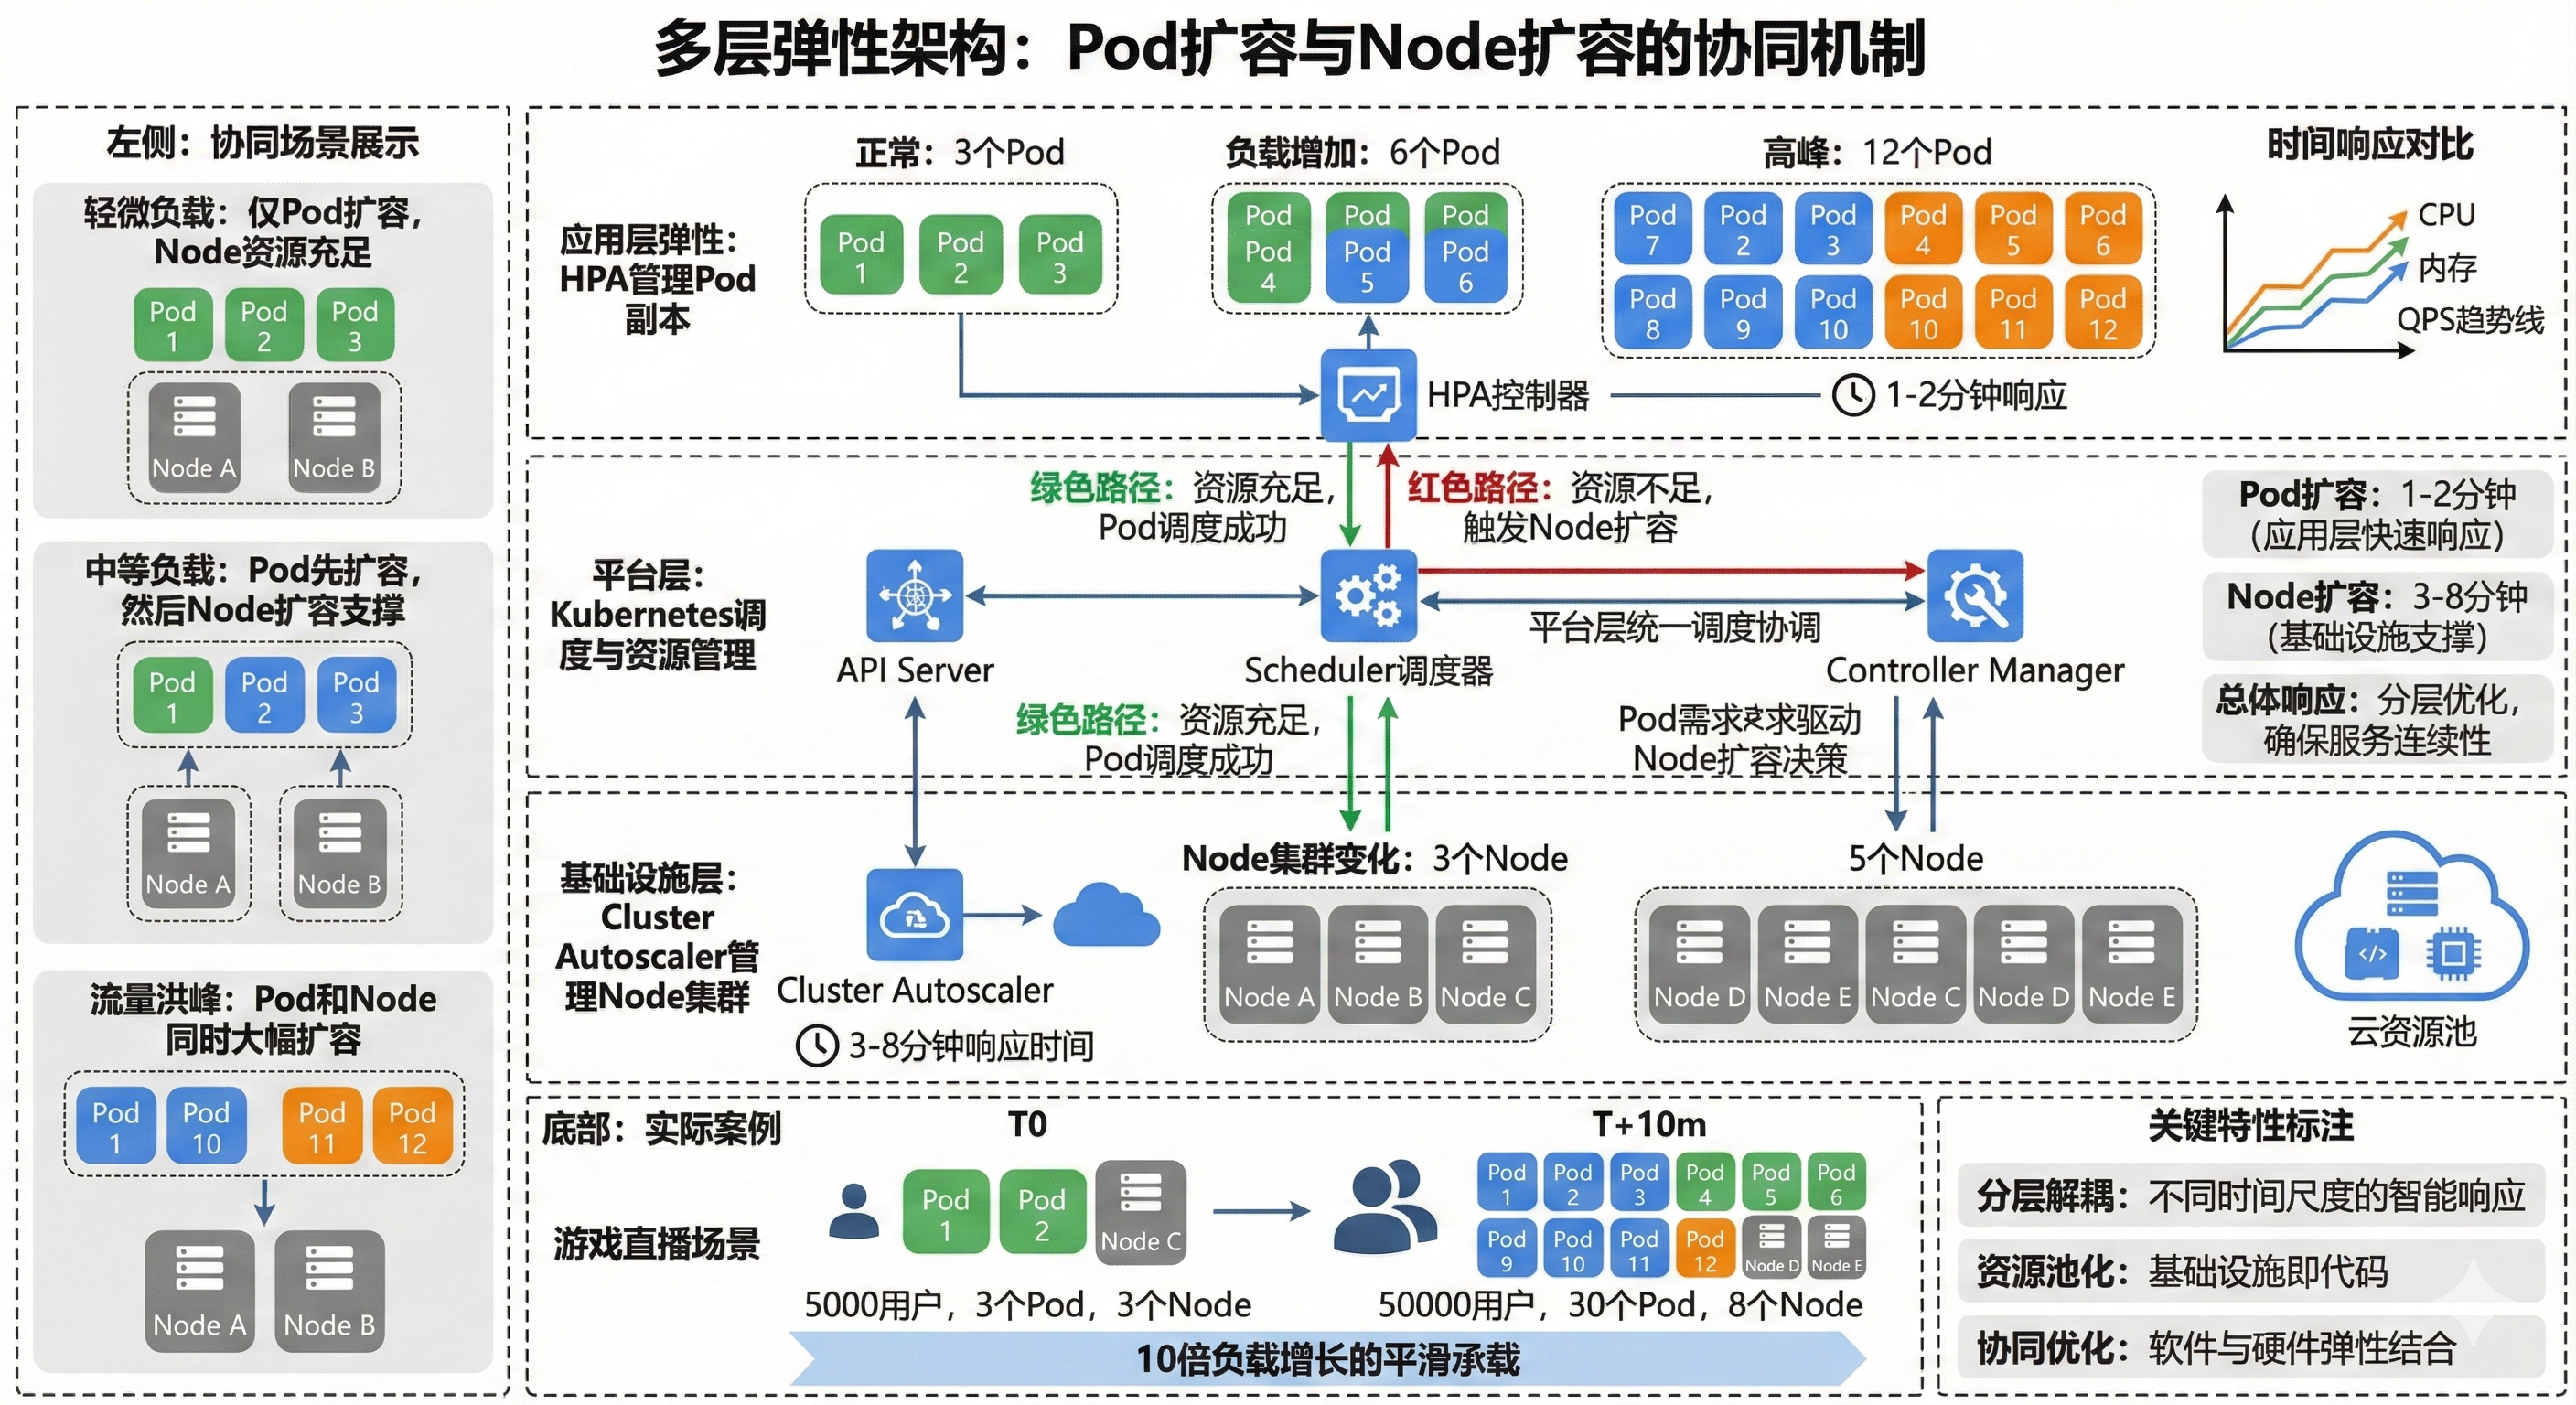
\includegraphics[width=0.9\textwidth]{figures/sec5/multi-layer-elasticity.png}
\caption{多层弹性架构：Pod扩容与Node扩容的协同}
\label{fig:multi-layer-elasticity}
\end{figure}

如图~\ref{fig:multi-layer-elasticity}所示，HPA与Cluster Autoscaler构成了两层弹性体系。HPA负责应用层的精细调度，响应速度快（1--2分钟），因为只需在现有Node上启停容器。Cluster Autoscaler负责基础设施层的宏观扩展，响应较慢（3--5分钟），因为涉及虚拟机的创建与初始化。两者配合，覆盖了从秒级到分钟级、从软件层到硬件层的弹性需求。

\subsubsection{成本经济学}

弹性扩容的价值不仅体现在技术层面，更直接反映在成本结构上。传统做法按峰值一次性采购服务器，平时常有70\%到80\%资源闲置。云上弹性按使用付费，但要做到"既省钱又稳"，关键在预留实例与按需实例的配比。

预留实例（Reserved Instance）通常比按需便宜30\%到60\%，代价是提前承诺容量与周期。按需实例（On-Demand）单价更高但调度最灵活。对游戏场景，建议把稳定底座（如长期在线的5000并发）放在预留实例上，把活动冲高部分（如从5000跃升到50000并发）交给按需实例承接。这种"基线预留加弹性按需"的策略相较纯按需常可降低40\%到60\%总云成本。竞价实例（Spot Instance）还能再便宜60\%到90\%，但可能被云厂商随时回收，适合非关键的离线批处理任务，不应承载实时对战的在线会话。

\subsection{Serverless：按调用付费的极致弹性}

\subsubsection{从K8s到Serverless：还能再省什么}

\begin{figure}[htbp]
\centering
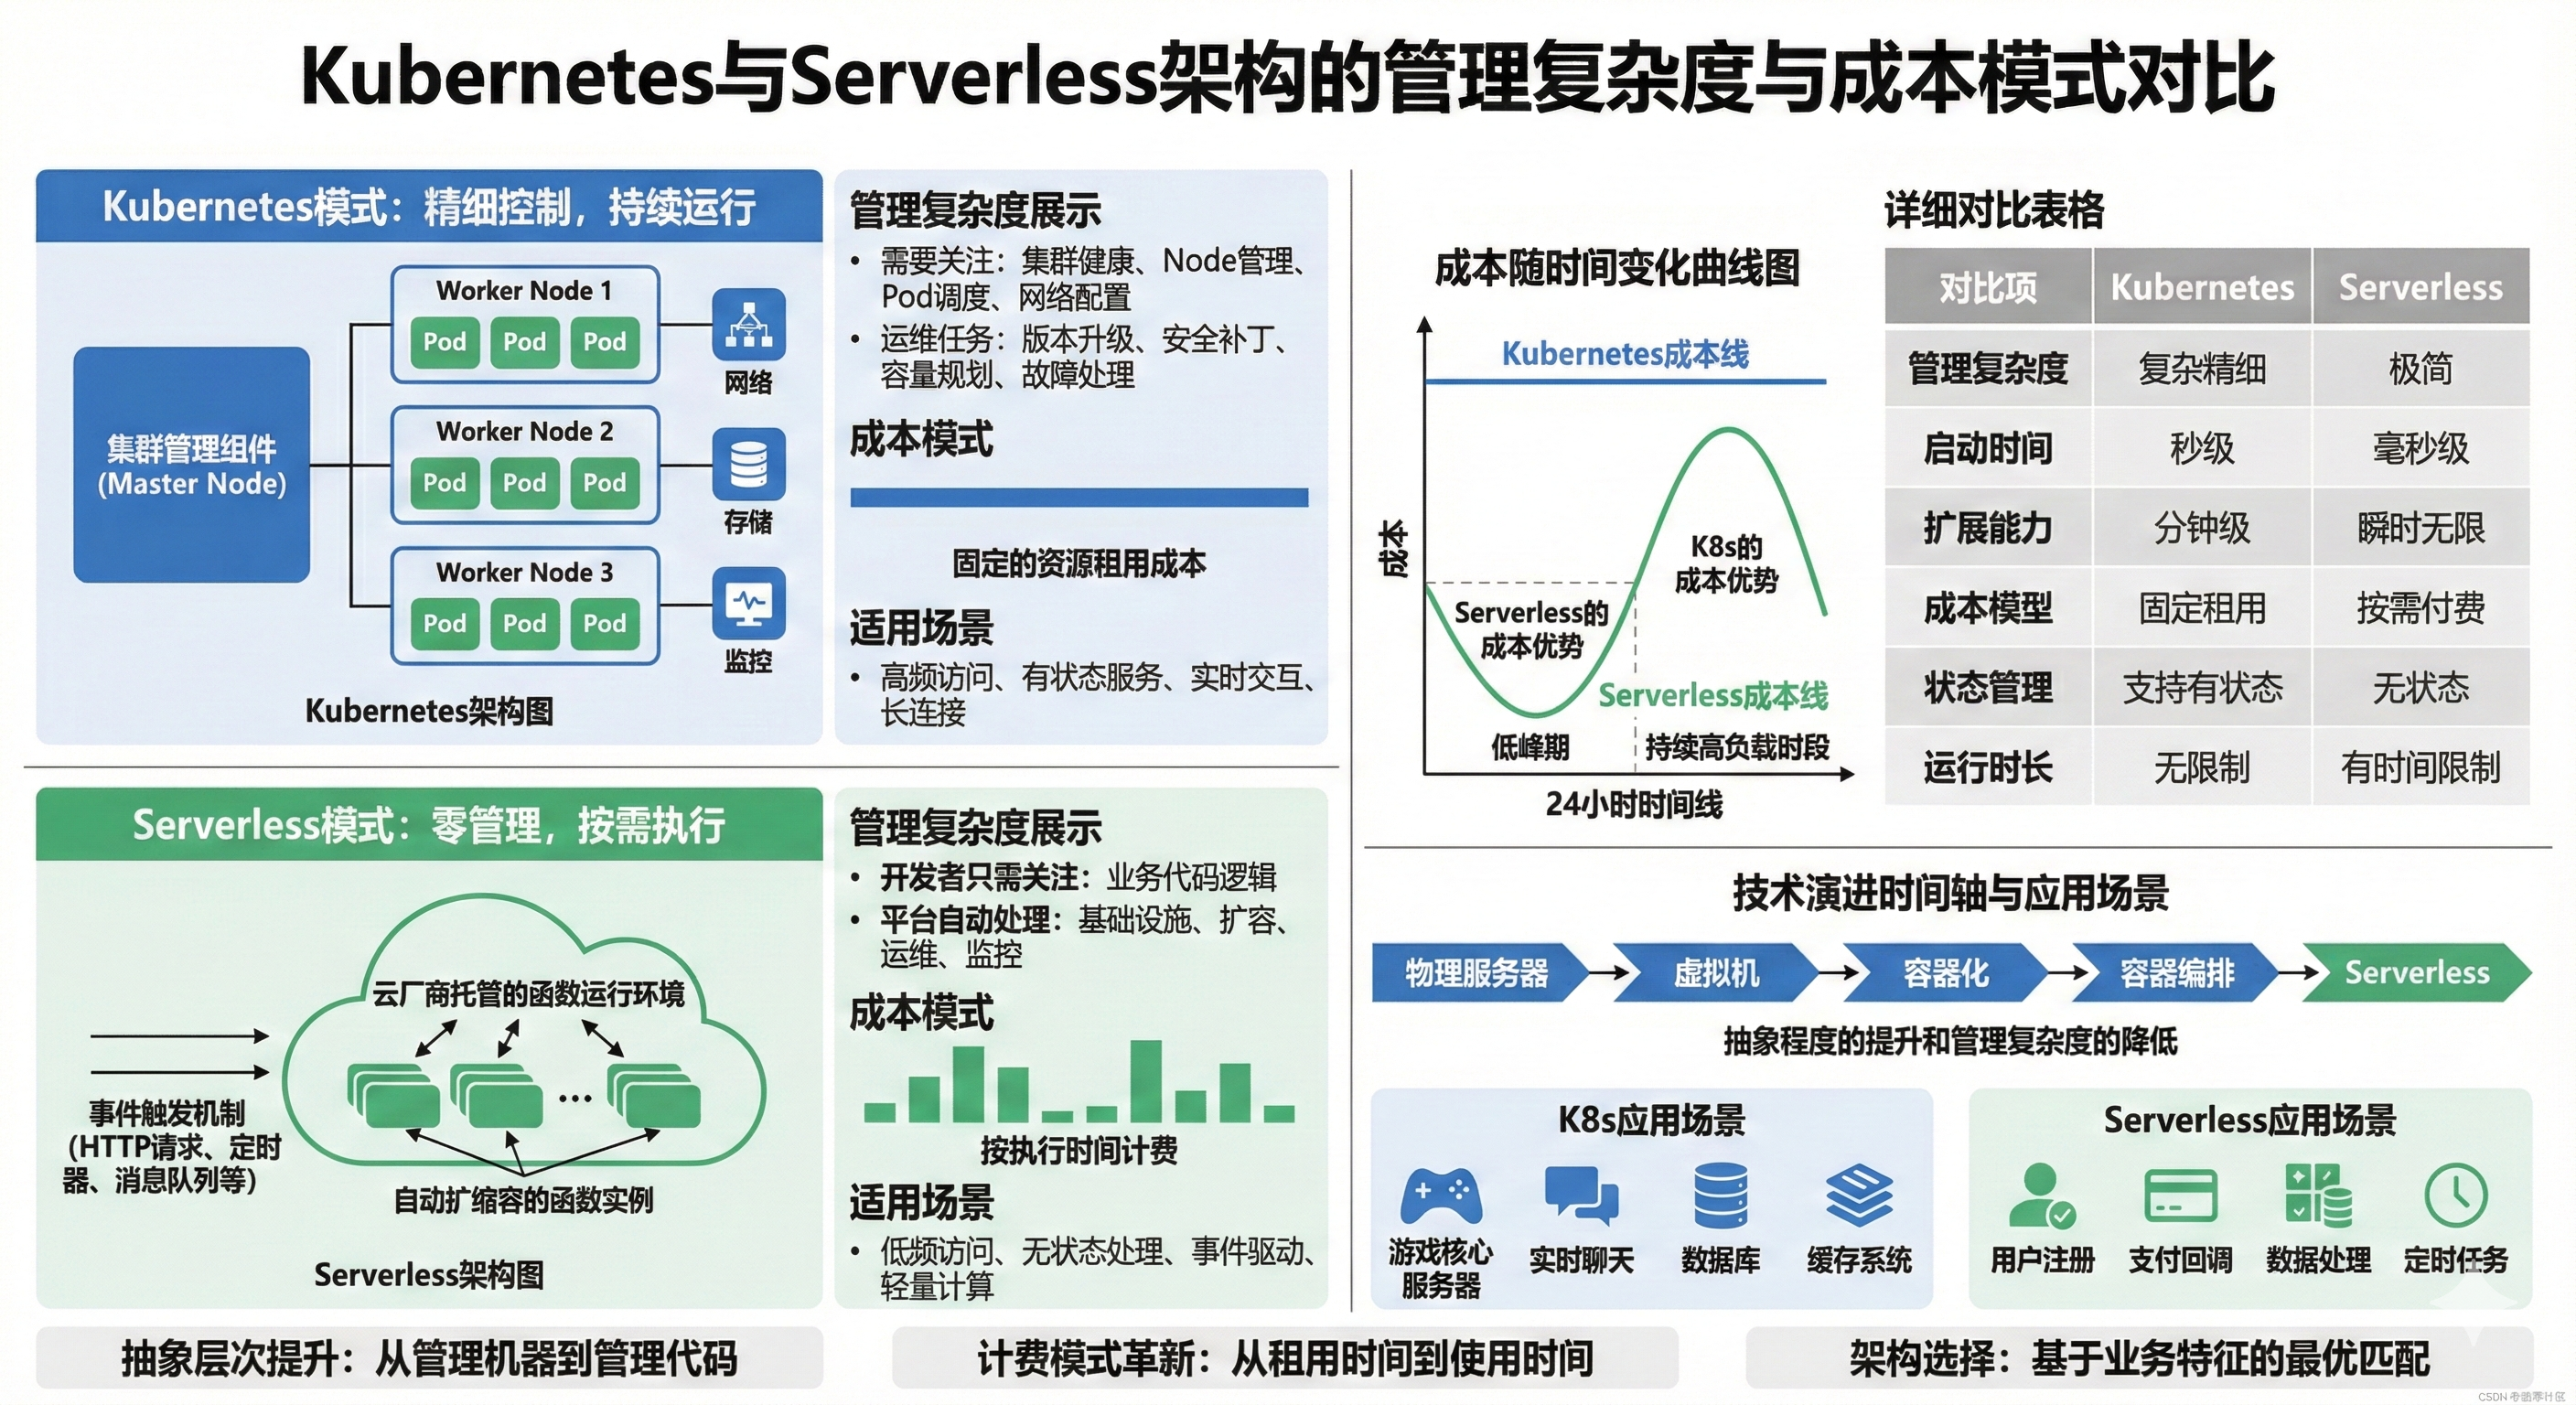
\includegraphics[width=0.9\textwidth]{figures/sec5/kubernetes-vs-serverless-comparison.png}
\caption{Kubernetes与Serverless的管理复杂度与成本模式对比}
\label{fig:k8s-vs-serverless}
\end{figure}

即使有了K8s的自动化编排和弹性伸缩，我们仍然需要关心集群的健康监控、Node的规格选择、网络安全配置等基础设施细节。对于游戏后端中那些低频、突发、轻量的辅助功能——每日签到、邮件系统、排行榜计算、活动奖励发放——专门维护一组常驻Pod显得过于沉重。

Serverless（无服务器）架构彻底抽象掉了服务器管理：你只需编写业务逻辑代码并部署到云平台，平台自动处理资源分配、弹性伸缩和故障恢复。更关键的是计费模式的变革：按代码实际运行时间收费，而非按服务器租用时间。如果没有玩家触发签到功能，代码不运行，费用为零。如图~\ref{fig:k8s-vs-serverless}所示，这种模式对具有明显波峰波谷特征的业务场景能带来显著的成本优势。

Serverless采用事件驱动的执行模型：函数按需启动，处理完请求后实例立即回收。这与K8s中Pod常驻内存、持续监听请求的模式形成鲜明对比。

\subsubsection{游戏场景的适用性分析}

\begin{table}[htbp]
\centering
\caption{Serverless与Kubernetes的场景化决策参考}
\label{tab:serverless-k8s-decision}
\begin{tabular}{|p{0.26\textwidth}|p{0.18\textwidth}|p{0.46\textwidth}|}
\hline
业务特征 & 推荐方案 & 主要原因 \\
\hline
长连接实时交互 & Kubernetes & WebSocket/TCP长连接需要稳定连接驻留，容器常驻模型更匹配 \\
\hline
有状态会话管理 & Kubernetes & 会话粘性、进程内状态与低抖动路由更容易在K8s中实现 \\
\hline
低频触发式任务 & Serverless & 按调用计费可避免空闲资源浪费，成本可下降90\%以上 \\
\hline
不可预测突发流量 & Serverless & 自动弹性能力强，能快速扩缩并减少人工容量规划压力 \\
\hline
定时批处理 & Serverless & 与事件调度天然契合，任务短平快且资源利用率高 \\
\hline
延迟敏感（$<$50\,ms） & Kubernetes & 冷启动尾延迟风险较高，常驻实例更容易保障严格时延目标 \\
\hline
\end{tabular}
\end{table}

Serverless并非适用于所有场景。如表~\ref{tab:serverless-k8s-decision}所示，核心游戏服务（实时对战、世界状态同步、聊天系统）需要维持长连接和管理复杂状态，仍然适合运行在K8s上。而周边辅助功能（用户注册、支付回调、数据分析、运营活动）通常具有无状态、低频次、可独立执行的特点，正好契合Serverless的优势。

\begin{figure}[htbp]
\centering
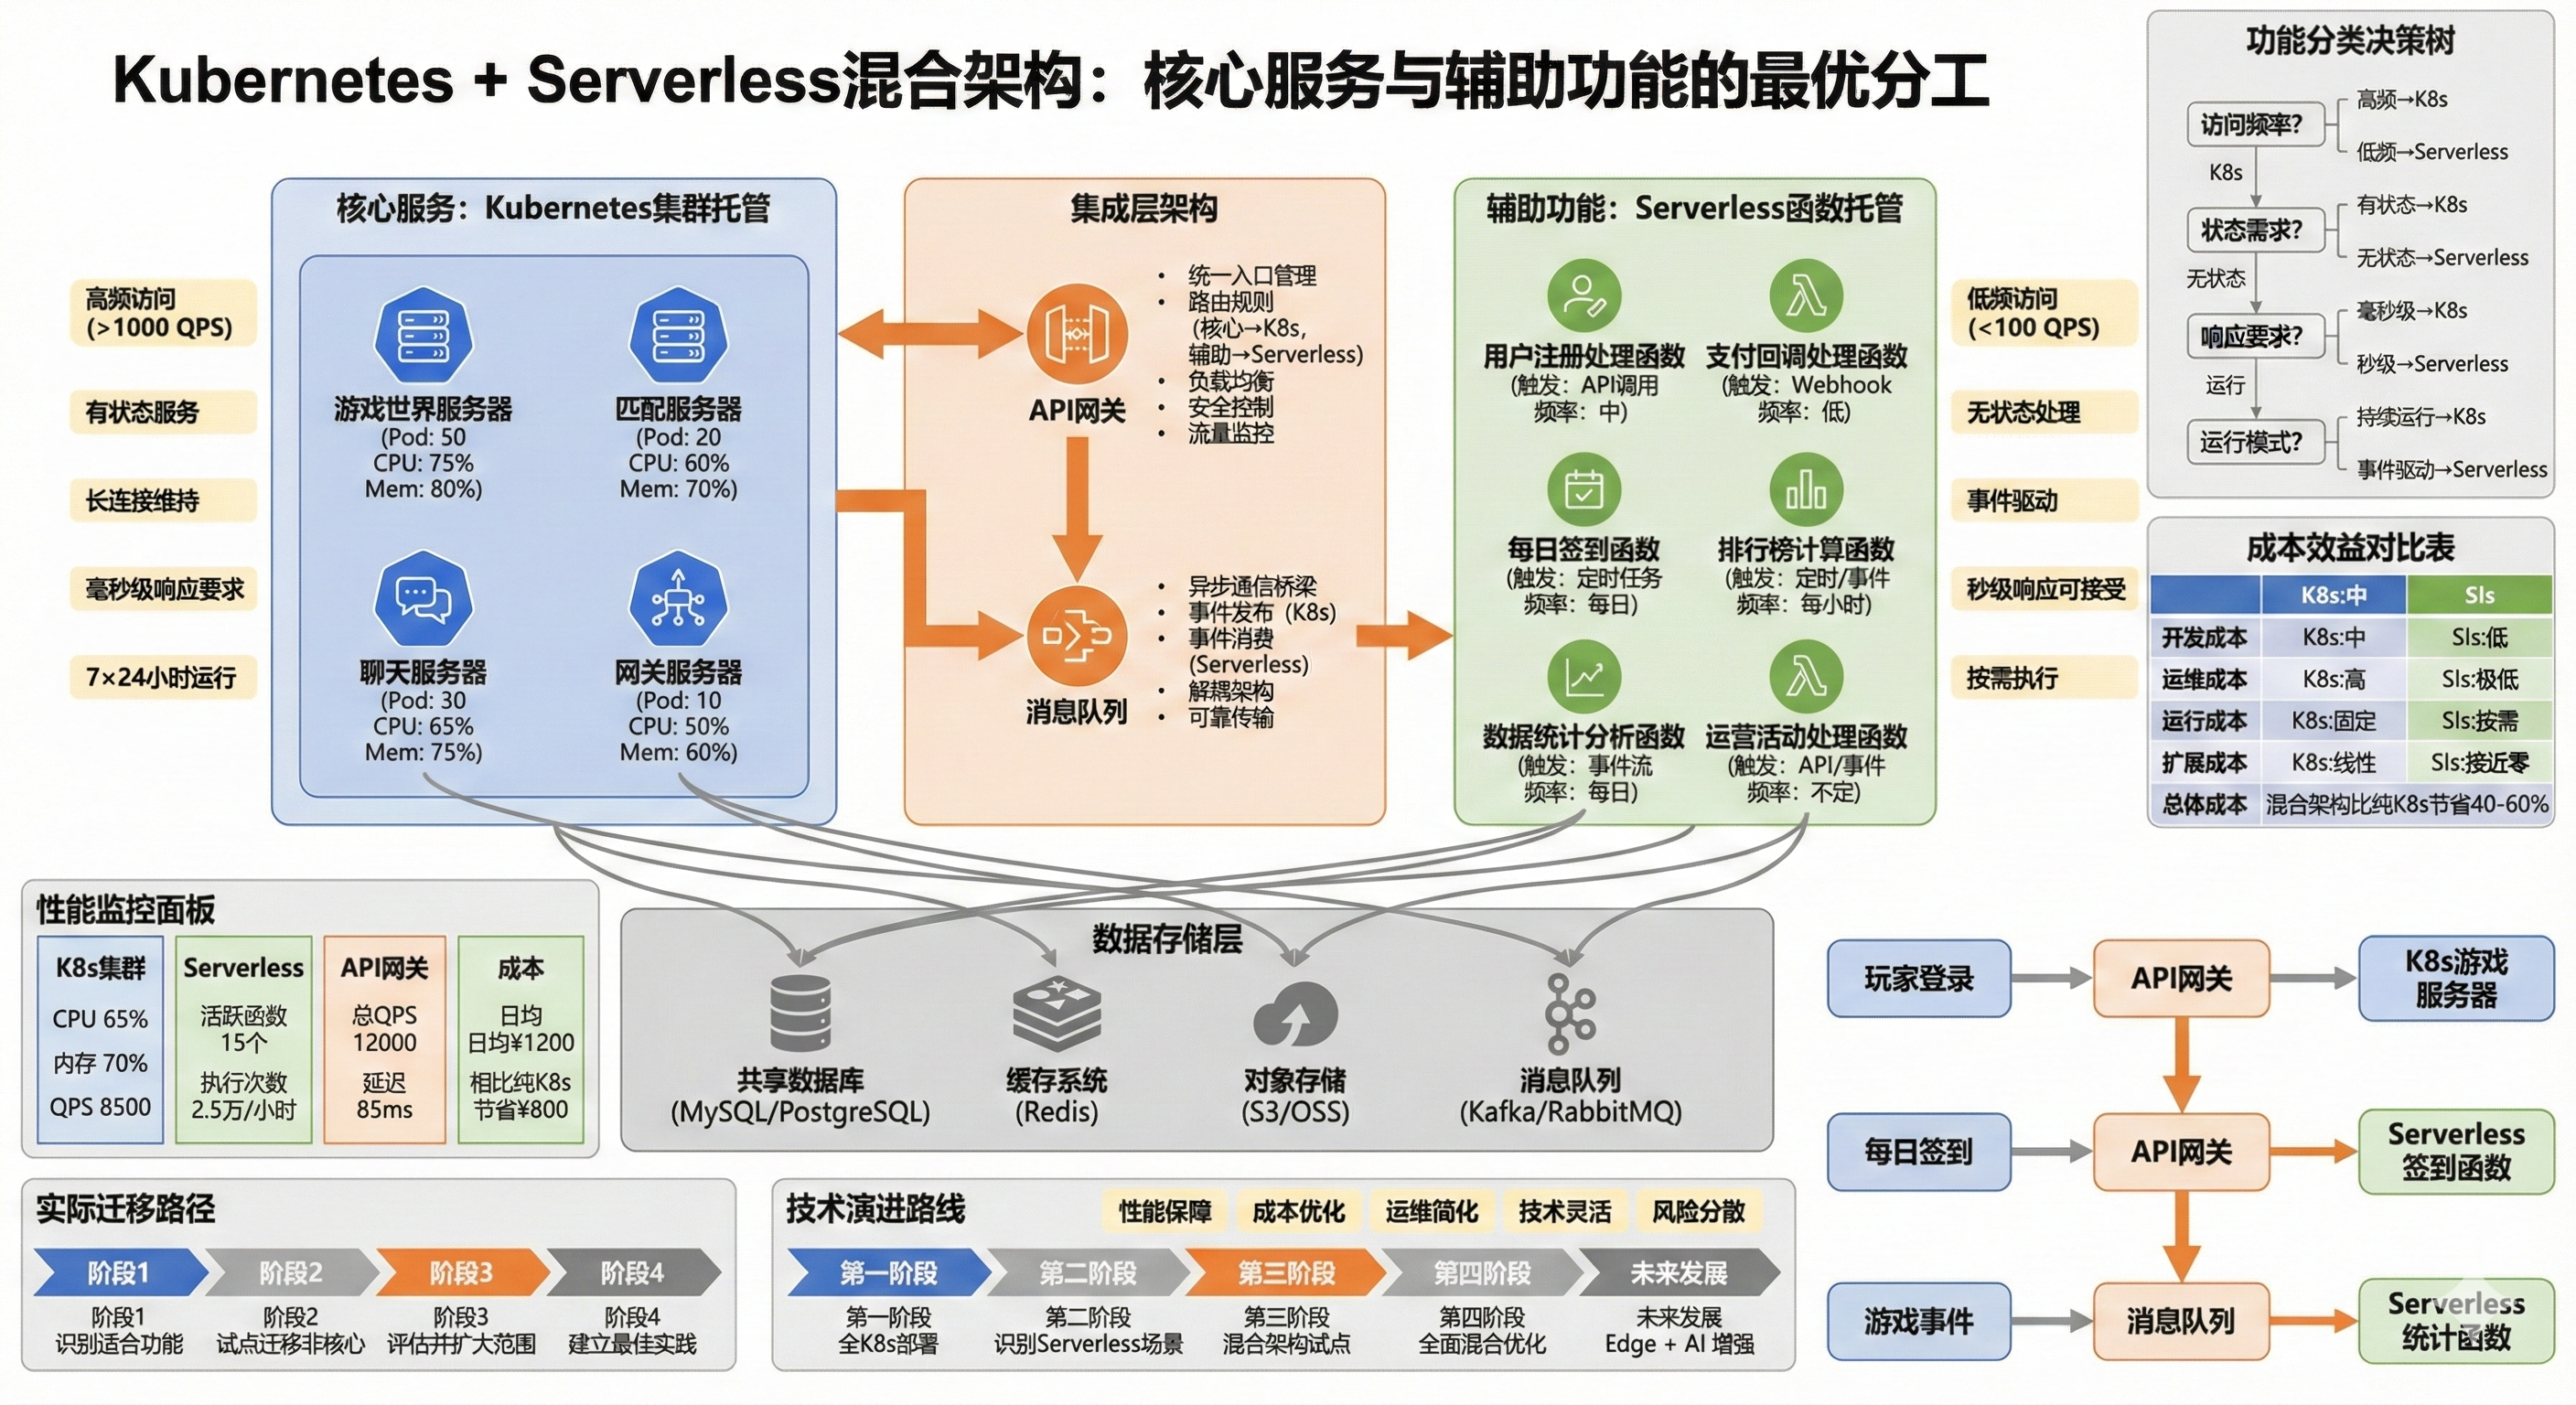
\includegraphics[width=0.9\textwidth]{figures/sec5/hybrid-architecture-design.png}
\caption{K8s + Serverless混合架构：核心服务与辅助功能的分工}
\label{fig:hybrid-architecture}
\end{figure}

如图~\ref{fig:hybrid-architecture}所示，实际项目中更常见的是混合架构：K8s集群承载核心游戏服务，Serverless函数处理辅助功能，两者通过API网关和消息队列集成。这种分层策略既保证了核心体验的稳定性，又充分利用了Serverless在成本和运维方面的优势。

\subsubsection{冷启动：Serverless的阿喀琉斯之踵}

\begin{figure}[htbp]
\centering
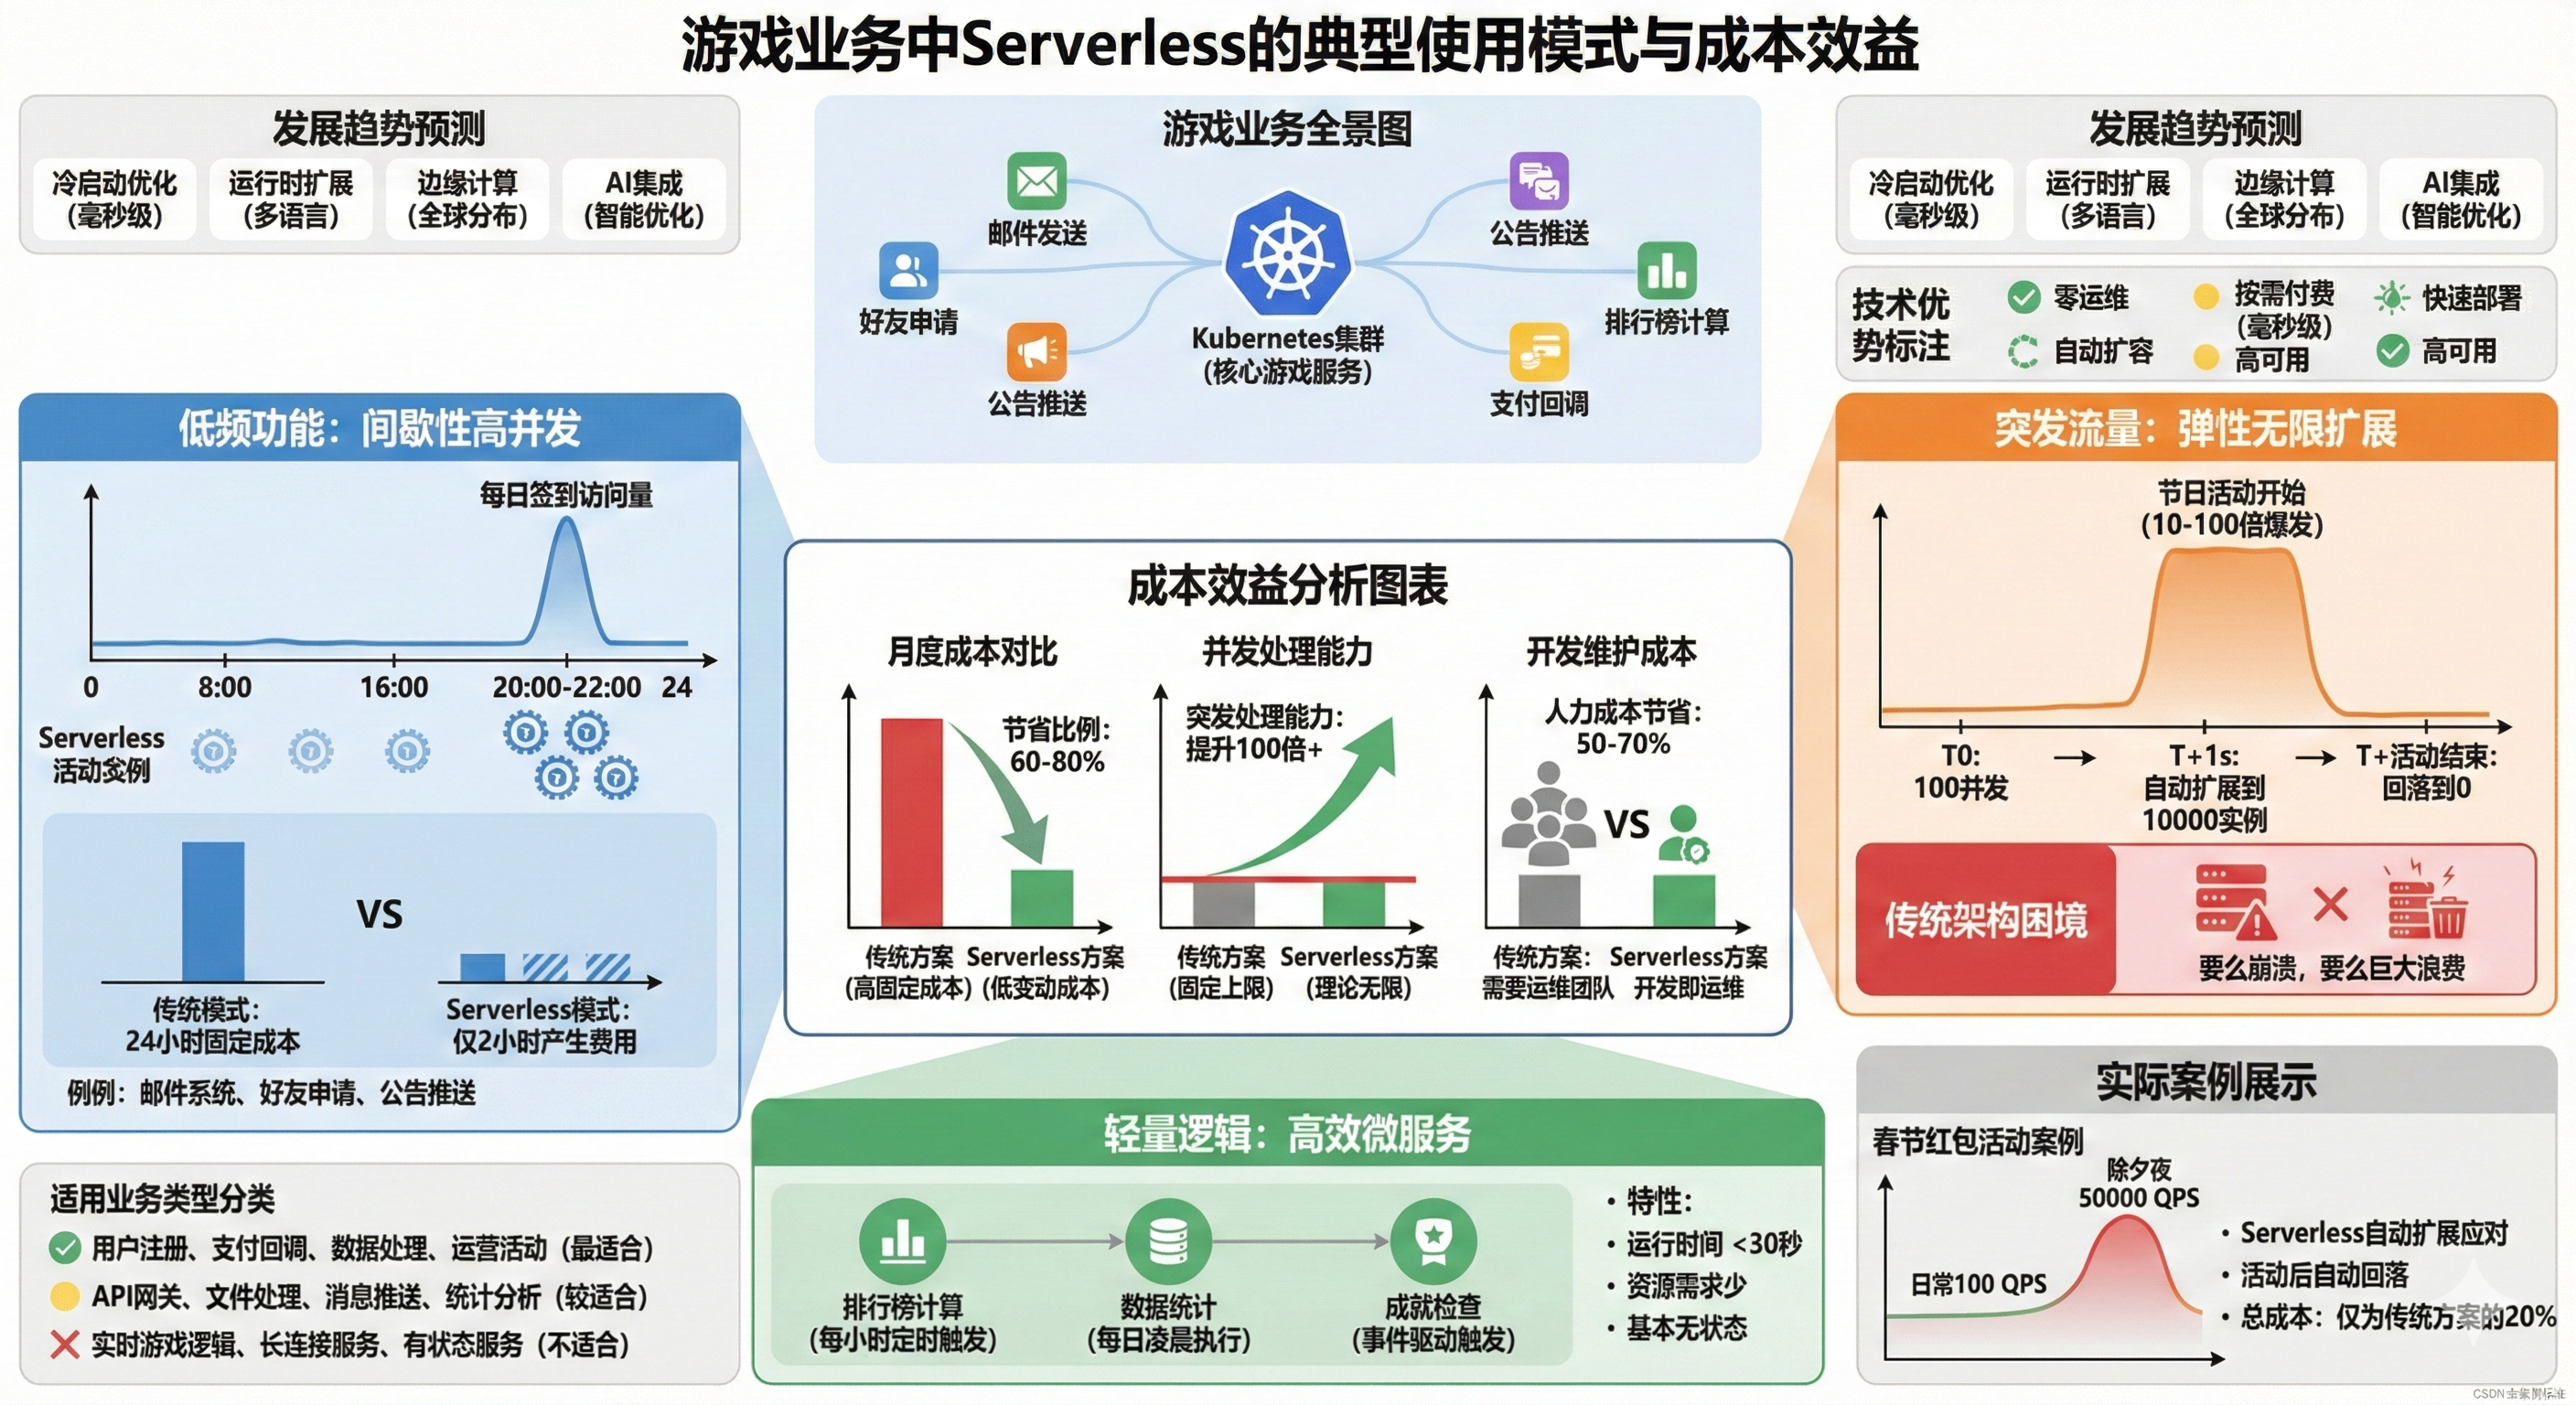
\includegraphics[width=0.9\textwidth]{figures/sec5/serverless-usage-patterns.png}
\caption{Serverless的典型使用模式与冷启动影响}
\label{fig:serverless-patterns}
\end{figure}

Serverless最被诟病的问题是冷启动延迟。当一个函数实例不存在时，平台需要从零创建执行环境，这个过程由多个串行阶段叠加而成。

第一阶段是执行环境创建：平台完成沙箱分配、网络与文件系统挂载等基础准备。在主流实现中，Firecracker microVM的启动时间约125\,ms，同时保持接近虚拟机级别的隔离性。第二阶段是运行时初始化：不同语言差异显著——Go与Rust的启动开销接近零，Python和Node.js增加几十到数百毫秒，传统JVM在类加载和JIT预热场景下可能增加秒级延迟。第三阶段是应用代码加载：依赖导入、数据库连接建立、配置读取等，这部分最受开发者控制。

工程上的优化重点应放在可控环节：对稳定高峰流量使用预留并发（Provisioned Concurrency）进行预热（但会增加常驻成本）；优先选择轻量运行时；JVM场景考虑GraalVM Native Image缩短启动路径；缩小部署包体积、减少无关依赖，并通过延迟加载将非首请求必需的逻辑后置。关于快照恢复（snapshot-restore）如何进一步压缩甚至消除冷启动，以及gVisor、Kata Containers等轻量虚拟化方案的原理对比，我们将在第六章展开。

\subsection{小结：从手工作坊到云原生工业}

本章的旅程，是一场被问题驱动的逐步演进。

起点是一个具体的工程困境：第四章设计好的分布式游戏后端，要部署到真实的云服务器上运行。我们首先遭遇了环境一致性问题——同一份代码换台机器就跑不了。比较了手工安装、虚拟机和容器三条路径后，我们选择了Docker：用镜像封装完整的运行环境，用分层构建实现高效复用，用Registry和摘要锁定实现可靠分发。

单个容器的问题解决后，多容器的协同启动成为新的痛点。Docker Compose通过声明式配置将手工操作收敛为一条命令，但它的能力边界止于单机。当我们需要跨多台机器调度容器、自动故障恢复和滚动更新时，Kubernetes接管了编排职责。K8s的核心价值在于声明式管理和持续调谐：你描述期望状态，系统自动逼近并维持。

有了集群编排能力后，"固定配置遇上波动流量"的成本矛盾浮出水面。HPA和Cluster Autoscaler构成的两层弹性体系，让资源能够跟着负载自动伸缩。而对于低频、突发、轻量的辅助功能，Serverless提供了按调用付费的极致弹性，与K8s形成互补的混合架构。

每一步都是被前一步的局限性逼出来的：环境不一致逼出了容器，多容器管理逼出了Compose，单机局限逼出了K8s，成本矛盾逼出了弹性伸缩，运维负担逼出了Serverless。这条演进路径不是人为设计的技术堆叠，而是工程实践中自然生长出来的解决方案链。

至此，我们的游戏架构已经从一个脆弱的本地原型，进化为一套能够根据流量自动伸缩、故障自动恢复的云原生系统。但我们目前掌握的是"驾驶"这辆云原生战车的能力——会用Docker封装、会用K8s编排、会配置弹性策略。当匹配服在晚高峰抖动、战斗服时延突增、灰度发布引发连锁故障时，只有理解系统内部的机理，才能做出稳定的技术判断。下一章，我们将真正打开引擎盖，深入容器隔离、调度算法、控制论、服务网格等底层原理。

\newpage